\documentclass[sigconf,nonacm]{acmart}

% === Packages ===
\usepackage{amsmath}
% amssymb omitted: \Bbbk conflicts with newtxmath in acmart
\usepackage{graphicx}
\usepackage{booktabs}
\usepackage{multirow}
\usepackage{subcaption}
\usepackage{xcolor}
\usepackage{tikz}
\usetikzlibrary{shapes,arrows,positioning,fit,calc,decorations.pathreplacing}
\usepackage{listings}
\usepackage{hyperref}
\usepackage{enumitem}
\usepackage{cleveref}

% === Listings style for Rust ===
% Rust language definition for listings
\lstdefinelanguage{Rust}{
  morekeywords={as, break, const, continue, crate, else, enum, extern, false,
    fn, for, if, impl, in, let, loop, match, mod, move, mut, pub, ref, return,
    self, Self, static, struct, super, trait, true, type, unsafe, use, where,
    while, async, await, dyn, abstract, become, box, do, final, macro,
    macro_rules, override, priv, try, typeof, unsized, virtual, yield},
  morekeywords=[2]{u8, u16, u32, u64, u128, i8, i16, i32, i64, i128,
    f32, f64, bool, char, str, String, Vec, Option, Result, Box, Rc, Arc,
    Duration, HashMap, DashMap, Self, pub, async, await, true, false},
  sensitive=true,
  morecomment=[l]{//},
  morecomment=[s]{/*}{*/},
  morestring=[b]",
  morestring=[b]',
}

\lstset{
  basicstyle=\ttfamily\scriptsize,
  keywordstyle=\color{blue}\bfseries,
  keywordstyle=[2]{\color{teal}\bfseries},
  commentstyle=\color{gray},
  stringstyle=\color{orange},
  breaklines=true,
  frame=single,
  language=Rust,
  numbers=left,
  numberstyle=\tiny\color{gray},
  xleftmargin=2em,
  framexleftmargin=1.5em,
}

% === Custom colors ===
\definecolor{nexa-blue}{RGB}{33,150,243}
\definecolor{nexa-green}{RGB}{76,175,80}
\definecolor{nexa-red}{RGB}{244,67,54}
\definecolor{nexa-orange}{RGB}{255,152,0}
\definecolor{nexa-purple}{RGB}{156,39,176}

% === Title ===
\title{Nexa-net: A Decentralized Agent Communication Network with Semantic Routing, Zero-Trust Identity, and Micro-Transaction Economy}

\author{Owen Zhang}
\affiliation{%
  \institution{Nexa-net Project}
  \city{Beijing}
  \country{China}
}

\begin{document}

% Abstract must be before \maketitle in acmart
\begin{abstract}
The proliferation of Large Language Model (LLM) agents has created an urgent need for decentralized, semantically-aware communication infrastructure. Existing agent frameworks rely on centralized platforms that introduce single-point failures, lack semantic routing, provide no economic incentives for service providers, and depend on fragile API-key authentication models. We present \textbf{Nexa-net}, a decentralized Agent communication network built on a four-layer architecture: (1) Identity \& Zero-Trust Layer using W3C-compatible Decentralized Identifiers (DIDs) with Ed25519/X25519 cryptography; (2) Semantic Discovery \& Routing Layer combining HNSW vector indexing with Kademlia DHT for intent-driven capability matching; (3) Transport \& Protocol Layer featuring a 12-byte binary frame format with streaming RPC and dynamic compression negotiation; and (4) Economy \& Micro-Transaction Layer implementing state channels with dual-signature MicroReceipts for high-frequency off-chain settlements at 9.9M TPS. The system is implemented as a non-invasive Sidecar Proxy in Rust, enabling agents to join the network without code modifications. Benchmark results demonstrate routing latency of 31\textmu s (3,200$\times$ better than the 100ms target), channel throughput of 9.9M TPS (990$\times$ target), and serialization throughput of 5.6M ops/s (56$\times$ target). The implementation includes 485 tests covering unit, integration, E2E, and property-based testing, alongside 45 Criterion benchmarks across 8 modules.
\end{abstract}

\maketitle

% === Sections via input files ===
\section{Introduction}

\subsection{The Agent Communication Crisis}

The rapid advancement of Large Language Models (LLMs) has catalyzed an explosion of autonomous agents---software entities that perceive, reason, and act independently. From OpenAI's GPT-based toolchains~\cite{openai2024swarm} to multi-agent orchestration frameworks like AutoGen~\cite{wu2023autogen} and CrewAI~\cite{crewai2024}, agents are increasingly expected to collaborate: translating documents, extracting metrics, summarizing research, and orchestrating complex workflows across organizational boundaries.

However, the infrastructure supporting agent-to-agent (A2A) communication remains fundamentally inadequate. Current approaches suffer from four critical limitations:

\textbf{Centralized dependency.} Most agent frameworks route communication through centralized APIs---OpenAI's platform, LangChain Hub~\cite{chase2022langchain}, or proprietary middleware. This creates single-point failures: when the central service goes down, all dependent agents become unreachable. The 2023 OpenAI API outage rendered thousands of production pipelines inoperative, exposing the fragility of this model.

\textbf{Semantic routing absence.} Traditional service discovery relies on DNS and exact URL matching~\cite{consul2015,etcd2016}. An agent seeking ``document translation with format preservation'' must know the precise endpoint of a translation service, rather than describing its intent and letting the infrastructure discover the best match. This forces human operators to manually configure service addresses---a process that is antithetical to autonomous operation.

\textbf{Economic incentive vacuum.} Decentralized networks cannot rely on free labor. When Agent A calls Agent B's translation service, who pays? Without a native micro-transaction mechanism~\cite{nakamoto2008bitcoin}, service providers lack economic motivation to offer high-quality capabilities, and consumers lack budget guardrails to prevent runaway recursive calls (e.g., Agent A $\rightarrow$ B $\rightarrow$ A $\rightarrow$ B $\ldots$).

\textbf{Insecure authentication.} API keys are the predominant authentication mechanism for machine-to-machine (M2M) communication. Yet API keys require human distribution, are vulnerable to leakage, and cannot support dynamic trust relationships between autonomous entities. A zero-trust architecture~\cite{nist2020zerotrust,ward2016beyondcorp} demands cryptographic identity verification at every interaction.

\subsection{Nexa-net: The Sidecar Proxy Approach}

Nexa-net addresses these four limitations through a \emph{non-invasive Sidecar Proxy} architecture. Inspired by the service mesh pattern~\cite{envoy2017,istio2018,linkerd2018} where Envoy/Istio proxies mediate microservice communication without modifying application code, Nexa-net deploys a lightweight proxy process alongside each agent. The agent treats the proxy as a local tool---\texttt{nexa\_network\_call}---and the proxy handles identity verification, semantic routing, protocol negotiation, encrypted transport, and economic settlement transparently.

This design philosophy yields a critical advantage: \emph{agents join the network without code modifications}. A LangChain agent, an AutoGen agent, or a custom Python script all connect through the same proxy interface, forming a heterogeneous yet interoperable network.

\subsection{Core Contributions}

This paper presents the following contributions:

\begin{enumerate}[label=\textbf{C\arabic*.}]
  \item \textbf{Four-layer decentralized agent network architecture.} We define a layered protocol stack---Identity \& Zero-Trust, Semantic Discovery \& Routing, Transport \& Protocol, Economy \& Micro-Transaction---where each layer provides self-contained services with clear interfaces, enabling independent evolution and replacement.

  \item \textbf{HNSW-based semantic routing algorithm.} We combine HNSW approximate nearest neighbor search~\cite{malkov2018hnsw} with Kademlia DHT~\cite{maymounkov2002kademlia} and a multi-factor scoring formula (semantic similarity $\times$ quality score $\times$ cost factor $\times$ load penalty $\times$ latency penalty) to enable intent-driven capability discovery that scales sub-linearly.

  \item \textbf{Ed25519 + state channel zero-trust micro-transaction mechanism.} We design a state channel lifecycle with dual-signature MicroReceipts~\cite{lightning2016} and SHA-256 hash chains, achieving 9.9M TPS for off-chain transfers while maintaining the balance invariant $b_A + b_B = \text{total\_deposit}$.

  \item \textbf{Complete Rust implementation with 485 tests and 45 benchmarks.} The system is implemented in Rust~\cite{rust2010} with Tokio async runtime~\cite{tokio2022}, DashMap lock-free concurrency~\cite{dashmap2022}, and ed25519-dalek cryptographic signatures~\cite{ed25519dalek2022}. The test suite covers unit (433), integration (31), E2E (10), HTTP E2E (5), and property-based (6) testing, while Criterion benchmarks~\cite{criterion2022} validate performance across 8 modules.
\end{enumerate}

\subsection{Paper Organization}

The remainder of this paper is organized as follows. Section~3 reviews related work across agent frameworks, P2P networks, semantic search, and micro-payment systems. Section~4 presents the system architecture overview. Sections~5--8 detail each of the four protocol layers. Sections~9--11 cover the Proxy/API, Security, and Storage subsystems. Sections~12 and~13 present the testing methodology and performance analysis. Section~14 discusses limitations and future directions, and Section~15 concludes.
\section{Background and Related Work}

\subsection{Agent Frameworks}

The landscape of agent orchestration frameworks has expanded rapidly with the maturation of LLM capabilities. \textbf{AutoGen}~\cite{wu2023autogen} introduced a multi-agent conversation framework where agents exchange messages through a centralized orchestrator. While flexible in defining agent roles and conversation patterns, AutoGen relies on a hub-and-spoke communication model where all messages route through the orchestrator, creating a bottleneck and single-point failure.

\textbf{CrewAI}~\cite{crewai2024} organizes agents into ``crews'' with defined roles, goals, and tools. Its sequential and hierarchical process flows provide structure, but again depend on a central crew manager for task delegation and result aggregation. CrewAI agents cannot discover each other dynamically or negotiate protocols independently.

\textbf{LangChain}~\cite{chase2022langchain} provides a composable toolkit for building LLM applications, including chains, agents, and memory modules. LangChain's agent executor pattern (observe $\rightarrow$ think $\rightarrow$ act $\rightarrow$ observe) is powerful for single-agent reasoning, but multi-agent coordination requires external orchestration via LangGraph---a stateful graph executor that still operates within a centralized process boundary.

\textbf{OpenAI Swarm}~\cite{openai2024swarm} is a lightweight experimental framework for multi-agent orchestration using routine handoffs and function calls. Swarm agents transfer control by returning ``handoff'' directives, but this mechanism operates within a single OpenAI API session, inheriting all the platform's latency, cost, and availability constraints.

\textbf{Microsoft Semantic Kernel}~\cite{microsoft2023semantickernel} integrates LLMs with conventional programming languages through a planner-connector pattern. While it supports native function invocation and plan execution, Semantic Kernel agents communicate through in-memory function calls rather than network protocols, limiting cross-organizational collaboration.

The common limitation across these frameworks is \emph{centralized communication}. No framework provides decentralized identity, semantic service discovery, or economic settlement---the three pillars required for autonomous agents to form a self-sustaining network without human intervention.

\subsection{Peer-to-Peer Networks}

\textbf{BitTorrent}~\cite{cohen2003bittorrent} pioneered incentive-driven P2P file sharing through its tit-for-tat piece exchange protocol. While BitTorrent demonstrates that economic incentives can sustain a decentralized network, its chunk-level bartering model is unsuitable for agent service payments, which require fine-grained token accounting rather than piece-for-piece exchange.

\textbf{IPFS}~\cite{benet2014ipfs} provides content-addressed distributed storage using a Merkle DAG structure and BitSwap incentive protocol. IPFS excels at static content distribution but lacks dynamic service discovery---an IPFS CID identifies fixed content, not a live service capability. IPFS also inherits BitSwap's limitation of content-level exchange rather than monetary settlement.

\textbf{Kademlia}~\cite{maymounkov2002kademlia} is the de facto standard DHT protocol, used in BitTorrent, IPFS, and Ethereum's devp2p network. Its XOR metric for node distance and iterative lookup procedure provide efficient $O(\log N)$ routing. Nexa-net adopts Kademlia's routing table structure for the Semantic DHT layer but extends it with vector-based semantic proximity---a Kademlia node is ``close'' not only in XOR distance but also in embedding-space similarity.

\textbf{Chord}~\cite{stoica2001chord} and \textbf{Pastry}~\cite{rowstron2001pastry} provide alternative DHT designs with consistent hashing and leaf-set routing, respectively. While these protocols offer strong theoretical guarantees, Kademlia's simplicity and wide deployment make it a more practical foundation for Nexa-net's DHT layer.

\subsection{Service Discovery}

\textbf{Consul}~\cite{consul2015} provides service discovery through DNS and HTTP interfaces, backed by a Raft~\cite{ongaro2014raft}-based consensus protocol for catalog consistency. Consul's service registration includes health checks and metadata tags, but tags are flat strings---there is no semantic matching mechanism. An agent must specify exact service names rather than describing its intent.

\textbf{etcd}~\cite{etcd2016} is a distributed key-value store used by Kubernetes for service discovery and configuration. etcd's watch-based notification system enables reactive service registration, but its key-based lookup model provides no semantic understanding of service capabilities.

Traditional DNS-based discovery (SRV records) operates at even lower semantic resolution, mapping domain names to IP:port pairs. None of these systems can answer the query: ``Find me the cheapest translation service that handles PDF format and outputs Chinese.''

\subsection{Semantic Search and Vector Indexing}

\textbf{HNSW}~\cite{malkov2018hnsw} (Hierarchical Navigable Small World) is the state-of-the-art approximate nearest neighbor (ANN) algorithm. Its multi-layer navigable small world graph structure achieves recall rates exceeding 95\% at query latencies of 25--46\textmu s for indexes of 100--10,000 vectors. Nexa-net's Semantic Router builds on HNSW for capability vector indexing, augmented with SIMD-optimized cosine distance computation in pure f32 arithmetic.

\textbf{FAISS}~\cite{johnson2019faiss} (Facebook AI Similarity Search) provides GPU-accelerated ANN search for billion-scale indexes. While FAISS excels at batch indexing and search on GPU hardware, its CPU-only mode lacks the low-latency single-query performance needed for real-time agent routing. HNSW offers superior single-query latency on CPU, making it more suitable for Nexa-net's proxy-side routing decisions.

\textbf{word2vec}~\cite{mikolov2013word2vec}, \textbf{BERT}~\cite{devlin2019bert}, and \textbf{sentence-transformers}~\cite{reimers2019sentence} provide the embedding models that transform text descriptions into high-dimensional vectors. Nexa-net's vectorizer module supports both a Mock embedder (for testing) and an ONNX Runtime~\cite{onnxruntime2021} embedder (for production), enabling 384-dimensional embeddings at 5.64\textmu s per text (mock) or production-grade latency with pre-trained sentence-BERT models.

\textbf{Annoy}~\cite{spotify2019annoy} and \textbf{ScaNN}~\cite{google2020scann} provide alternative ANN implementations. Annoy uses random projection trees for static indexes, while ScaNN achieves higher throughput through anisotropic quantization. For Nexa-net's use case---dynamic indexes where capabilities are registered and unregistered frequently---HNSW's support for incremental insertion makes it the clear choice over static-index approaches.

\subsection{Micro-Payment Systems}

\textbf{Bitcoin Lightning Network}~\cite{lightning2016} pioneered the state channel concept for Bitcoin, enabling off-chain micropayments with on-chain settlement guarantees. Lightning's Hash-Time-Locked Contracts (HTLCs) provide atomic routing across multiple hops, but its channel opening requires on-chain transactions (10+ minute confirmation time), making it unsuitable for the rapid channel establishment needed in agent networks.

\textbf{Raiden Network}~\cite{raiden2017} extends state channels to Ethereum~\cite{buterin2014ethereum}, supporting ERC-20 token transfers with mediated paths. Raiden shares Lightning's limitation of on-chain channel opening, but its smart contract flexibility allows more sophisticated settlement conditions.

Nexa-net's state channel design draws from Lightning and Raiden's architectural patterns but operates at a different abstraction level. Rather than anchoring channels to a blockchain, Nexa-net channels are anchored to \emph{cryptographic receipts}---each MicroReceipt carries dual Ed25519 signatures and a SHA-256 hash chain link. Settlement occurs when the channel closes and the final state is submitted to a SettlementEngine. This approach trades on-chain verifiability for latency optimization, achieving 9.9M TPS compared to Lightning's theoretical 10K TPS.

\subsection{Zero-Trust and SPIFFE}

\textbf{SPIFFE}~\cite{spiffe2020} (Secure Production Identity Framework for Everyone) defines a standard for service identity in dynamic environments. SPIFFE's SVID (X.509 certificate + URI SAN) model is conceptually aligned with Nexa-net's DID-based identity, but SPIFFE assumes a centralized Workload API that attests identities---a design that conflicts with Nexa-net's self-sovereign identity principle where agents generate and control their own DIDs without a central attestation authority.

\textbf{BeyondCorp}~\cite{ward2016beyondcorp} (Google's zero-trust implementation) shifts access validation from network perimeter to individual device and user identity. While BeyondCorp demonstrates that zero-trust is feasible at enterprise scale, it depends on Google's internal identity federation---a centralized trust anchor. Nexa-net distributes trust anchors across multiple independent entities, requiring only DID Document signature verification rather than centralized attestation.

\textbf{NIST Zero Trust Architecture}~\cite{nist2020zerotrust} (SP 800-207) formalizes zero-trust principles: never trust, always verify; least privilege access; assume breach. Nexa-net implements all three principles: every RPC call requires DID verification and mTLS; Verifiable Credentials~\cite{w3c_vc_2022} enforce least privilege; and the AuditLogger records all interactions for post-breach forensics.

\subsection{Sidecar Proxy and Service Mesh}

\textbf{Envoy}~\cite{envoy2017} pioneered the sidecar proxy pattern for microservice communication, providing L7 load balancing, mTLS termination, and observability without application code changes. \textbf{Istio}~\cite{istio2018} orchestrates Envoy sidecars through a centralized control plane (Pilot for routing, Citadel for identity, Galley for config). \textbf{Linkerd}~\cite{linkerd2018} offers a lighter-weight alternative with similar sidecar architecture.

Nexa-net adopts the sidecar pattern from service mesh literature but diverges in three key aspects: (1) the proxy handles \emph{semantic routing} rather than URL-based load balancing; (2) the proxy implements \emph{economic settlement}---no service mesh charges for API calls; (3) the proxy uses \emph{decentralized identity} (DID) rather than centralized certificate authority (Istio Citadel).

\subsection{DID and Verifiable Credentials}

\textbf{W3C DID Core}~\cite{w3c_did_2022} defines a universal identifier format (\texttt{did:method:identifier}) with resolution to DID Documents containing verification methods, service endpoints, and key agreement protocols. Nexa-net's DID implementation (\texttt{did:nexa:<hex>}) follows W3C DID syntax with Ed25519 verification keys and X25519 key agreement keys.

\textbf{W3C Verifiable Credentials}~\cite{w3c_vc_2022} provide a standard for expressing credentials with cryptographic proofs of issuer authenticity. Nexa-net uses VCs for capability attestation---a Trust Anchor issues a VC confirming that a service provider's claimed capabilities (e.g., ``translation accuracy 0.95'' or ``latency 2000ms'') have been verified. This creates a trust chain from the agent's DID to its claimed capabilities without requiring a central registry.
\section{System Architecture Overview}

\subsection{Design Philosophy}

Nexa-net's architecture follows three guiding principles: \emph{non-invasive integration}, \emph{semantic-first routing}, and \emph{layered decomposition}. The non-invasive principle dictates that agents interact with Nexa-net through a local proxy---the agent merely calls \texttt{nexa\_network\_call(intent, data)} as a regular function, while the proxy transparently handles identity, discovery, transport, and economy. The semantic-first principle mandates that agents describe \emph{what they want} rather than \emph{where to find it}. The layered decomposition principle ensures that each protocol layer is self-contained with well-defined interfaces, following the OSI model's separation-of-concerns approach.

\subsection{Four-Layer Architecture}

Nexa-net's protocol stack comprises four layers, each addressing a distinct aspect of decentralized agent communication. Figure~\ref{fig:four-layer} illustrates the architecture.

\begin{figure}[t]
\centering
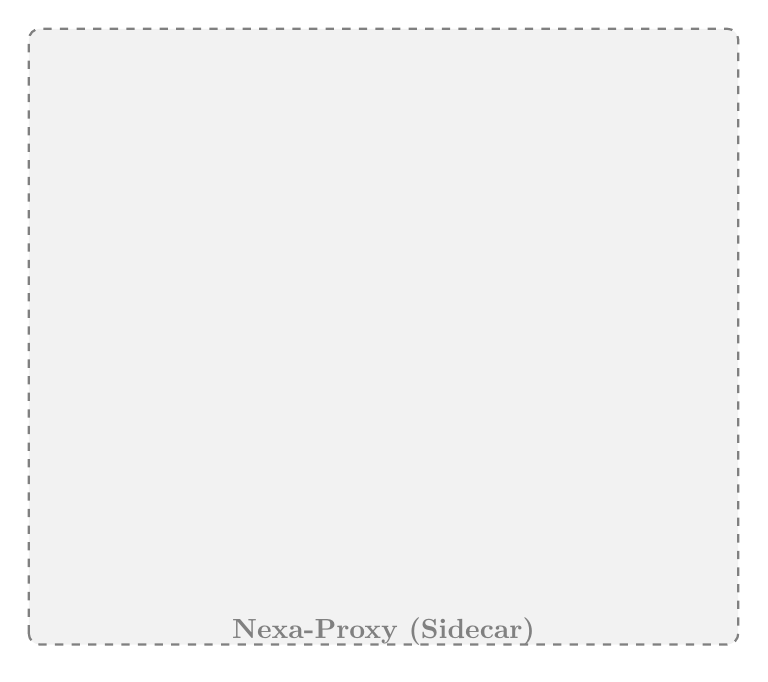
\begin{tikzpicture}[scale=0.85, every node/.style={font=\small}]
  % Layer 4 - Economy
  \draw[fill=nexa-orange!20, draw=nexa-orange, thick, rounded corners] (0,0) rectangle (10,2);
  \node[font=\normalsize\bfseries] at (5,1.7) {Layer 4: Economy \& Micro-Transaction};
  \node[font=\scriptsize] at (2.5,0.8) {State Channel};
  \node[font=\scriptsize] at (5,0.8) {MicroReceipt};
  \node[font=\scriptsize] at (7.5,0.8) {Token Engine};

  % Layer 3 - Transport
  \draw[fill=nexa-blue!20, draw=nexa-blue, thick, rounded corners] (0,2.2) rectangle (10,4.2);
  \node[font=\normalsize\bfseries] at (5,3.9) {Layer 3: Transport \& Protocol};
  \node[font=\scriptsize] at (2.5,3.0) {Handshake};
  \node[font=\scriptsize] at (5,3.0) {Streaming RPC};
  \node[font=\scriptsize] at (7.5,3.0) {Serialization};

  % Layer 2 - Discovery
  \draw[fill=nexa-green!20, draw=nexa-green, thick, rounded corners] (0,4.4) rectangle (10,6.4);
  \node[font=\normalsize\bfseries] at (5,6.1) {Layer 2: Semantic Discovery \& Routing};
  \node[font=\scriptsize] at (2.5,5.2) {Capability Schema};
  \node[font=\scriptsize] at (5,5.2) {Semantic Router};
  \node[font=\scriptsize] at (7.5,5.2) {DHT};

  % Layer 1 - Identity
  \draw[fill=nexa-purple!20, draw=nexa-purple, thick, rounded corners] (0,6.6) rectangle (10,8.6);
  \node[font=\normalsize\bfseries] at (5,8.3) {Layer 1: Identity \& Zero-Trust};
  \node[font=\scriptsize] at (2.5,7.4) {Nexa-DID};
  \node[font=\scriptsize] at (5,7.4) {mTLS};
  \node[font=\scriptsize] at (7.5,7.4) {VC};

  % Sidecar Proxy wrapper
  \draw[fill=gray!10, draw=gray, dashed, thick, rounded corners] (-0.3,-0.3) rectangle (10.3,8.9);
  \node[font=\normalsize\bfseries, color=gray] at (5,-0.1) {Nexa-Proxy (Sidecar)};
\end{tikzpicture}
\caption{Nexa-net four-layer architecture with Sidecar Proxy boundary.}
\label{fig:four-layer}
\end{figure}

\textbf{Layer 1 (Identity \& Zero-Trust)} establishes cryptographic identity through W3C-compatible DIDs with Ed25519 signing and X25519 key agreement. Every agent generates a \texttt{did:nexa:<hex>} identifier derived from SHA-256 of its Ed25519 public key, and publishes a DID Document containing verification methods and service endpoints. mTLS provides bidirectional authentication during connection establishment, and Verifiable Credentials enable capability attestation through a Trust Anchor chain.

\textbf{Layer 2 (Semantic Discovery \& Routing)} transforms textual intent descriptions into 384-dimensional embedding vectors and indexes them in HNSW for sub-linear search. The Kademlia DHT distributes the routing table across the network, and the Semantic Router combines similarity scores with quality, cost, load, and latency factors into a multi-factor scoring formula to select optimal service providers.

\textbf{Layer 3 (Transport \& Protocol)} implements a 12-byte binary frame format for efficient RPC communication, supporting four RPC patterns (Unary, Server-Stream, Client-Stream, Bidirectional). The SYN-NEXA/ACK-SCHEMA handshake negotiates protocol version, compression algorithm, and estimated cost before the first RPC call. Serialization supports JSON with LZ4/Zstd/Gzip compression pipelines.

\textbf{Layer 4 (Economy \& Micro-Transaction)} manages state channels between paired agents, tracking off-chain transfers with dual-signature MicroReceipts and SHA-256 hash chains. BudgetController enforces per-call, per-channel, and per-agent budget limits to prevent resource abuse. SettlementEngine computes final balances when channels close, maintaining the invariant $b_A + b_B = \text{total\_deposit}$.

\subsection{Sidecar Proxy Design}

The Sidecar Proxy pattern, borrowed from service mesh architecture~\cite{envoy2017,istio2018}, is central to Nexa-net's non-invasive philosophy. Each agent runs a Nexa-Proxy process on the same host (or container), listening on a local port for agent requests. The proxy encapsulates all four layers in a single \texttt{ProxyState} container that holds references to the DID resolver, semantic router, RPC engine, and channel manager.

\begin{figure}[t]
\centering
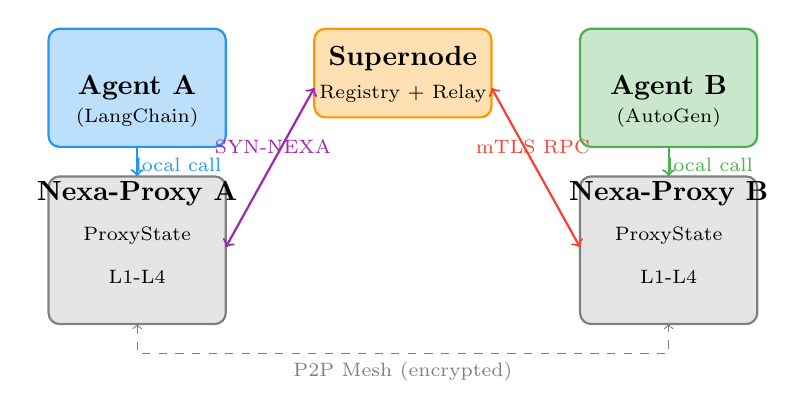
\begin{tikzpicture}[scale=0.75, every node/.style={font=\small}]
  % Agent A
  \draw[fill=nexa-blue!30, draw=nexa-blue, thick, rounded corners] (0,3) rectangle (3,5);
  \node[font=\bfseries] at (1.5,4) {Agent A};
  \node[font=\scriptsize] at (1.5,3.5) {(LangChain)};

  % Proxy A
  \draw[fill=gray!20, draw=gray, thick, rounded corners] (0,0) rectangle (3,2.5);
  \node[font=\bfseries] at (1.5,2.2) {Nexa-Proxy A};
  \node[font=\scriptsize] at (1.5,1.5) {ProxyState};
  \node[font=\scriptsize] at (1.5,0.8) {L1-L4};

  % Agent B
  \draw[fill=nexa-green!30, draw=nexa-green, thick, rounded corners] (9,3) rectangle (12,5);
  \node[font=\bfseries] at (10.5,4) {Agent B};
  \node[font=\scriptsize] at (10.5,3.5) {(AutoGen)};

  % Proxy B
  \draw[fill=gray!20, draw=gray, thick, rounded corners] (9,0) rectangle (12,2.5);
  \node[font=\bfseries] at (10.5,2.2) {Nexa-Proxy B};
  \node[font=\scriptsize] at (10.5,1.5) {ProxyState};
  \node[font=\scriptsize] at (10.5,0.8) {L1-L4};

  % Supernode
  \draw[fill=nexa-orange!30, draw=nexa-orange, thick, rounded corners] (4.5,3.5) rectangle (7.5,5);
  \node[font=\bfseries] at (6,4.5) {Supernode};
  \node[font=\scriptsize] at (6,3.9) {Registry + Relay};

  % Connections
  \draw[->, thick, nexa-blue] (1.5,3) -- (1.5,2.5);
  \node[font=\scriptsize, color=nexa-blue] at (2.2,2.7) {local call};

  \draw[->, thick, nexa-green] (10.5,3) -- (10.5,2.5);
  \node[font=\scriptsize, color=nexa-green] at (11.2,2.7) {local call};

  \draw[<->, thick, nexa-purple] (3,1.3) -- (4.5,4);
  \node[font=\scriptsize, color=nexa-purple] at (3.8,3) {SYN-NEXA};

  \draw[<->, thick, nexa-red] (7.5,4) -- (9,1.3);
  \node[font=\scriptsize, color=nexa-red] at (8.2,3) {mTLS RPC};

  \draw[<->, dashed, gray] (1.5,0) -- (1.5,-0.5) -- (10.5,-0.5) -- (10.5,0);
  \node[font=\scriptsize, color=gray] at (6,-0.8) {P2P Mesh (encrypted)};
\end{tikzpicture}
\caption{Agent--Proxy--Supernode interaction model. Each agent communicates with its local proxy; proxies negotiate with the supernode for discovery and with peer proxies for direct RPC.}
\label{fig:proxy-model}
\end{figure}

The data flow for a typical agent request proceeds as follows (Figure~\ref{fig:proxy-model}): (1) Agent A calls \texttt{nexa\_network\_call("translate PDF", data)} on its local proxy; (2) Proxy A vectorizes the intent and queries the Semantic DHT for matching capabilities; (3) The DHT returns ranked candidates via the Semantic Router; (4) Proxy A initiates a SYN-NEXA handshake with Proxy B (the selected service provider's proxy); (5) Proxies negotiate compression, budget, and protocol version; (6) Proxy A opens a state channel with Proxy B for payment; (7) The RPC call is executed over mTLS with compressed serialization; (8) A MicroReceipt is signed by both proxies, and the channel balance is updated; (9) The result is returned to Agent A through its local proxy.

\subsection{Component Interactions}

The four layers interact through well-defined interfaces. Layer 1 provides DID resolution and VC verification services that Layers 2--4 consume for authentication. Layer 2 provides capability lookup services that Layer 3 uses to select communication targets. Layer 3 provides the RPC transport that Layer 4 uses for receipt exchange. This cascading dependency ensures that upper layers can function only when lower layers have established their guarantees---a form of protocol-level guard clause that enforces the zero-trust principle at every layer boundary.
\section{Layer 1: Identity and Zero-Trust}

\subsection{Nexa-DID: W3C-Compatible Decentralized Identifiers}

Nexa-net implements a W3C DID Core~\cite{w3c_did_2022}-compatible identifier system called Nexa-DID. The identifier format follows the standard three-part structure:

\begin{equation}
\texttt{did:nexa:<identifier>} \quad \text{where} \quad \text{identifier} = \text{hex}(\text{SHA-256}(\text{pk}_{\text{Ed25519}})[0:40])
\end{equation}

The identifier is derived deterministically from the agent's Ed25519 public key using SHA-256 truncated to the first 40 bytes, encoded in hexadecimal. This approach ensures that: (1) the DID is globally unique, as different Ed25519 keys produce different hashes with negligible collision probability; (2) the DID is self-certifying, as anyone who knows the public key can verify the DID derivation; and (3) the DID is permanent, as the identifier does not change unless the agent's fundamental identity key is rotated.

The DID generation algorithm benchmarks at 18.71\textmu s for Ed25519 keypair generation and 9.75\textit{ns} for DID string parsing (validation of the \texttt{did:nexa:<hex>} format), making identity operations negligible overhead compared to the 31\textmu s semantic routing latency.

\subsection{DID Document Structure}

Each Nexa-DID resolves to a DID Document conforming to the W3C specification. The document includes:

\begin{itemize}
  \item \texttt{verificationMethod}: An Ed25519 public key entry with type \texttt{Ed25519VerificationKey2020}, used for message signing and authentication.
  \item \texttt{keyAgreement}: An X25519 public key entry with type \texttt{X25519KeyAgreementKey2020}, used for Diffie-Hellman key exchange during mTLS session establishment.
  \item \texttt{authentication}: A reference to the Ed25519 verification method, indicating that the DID controller can authenticate using this key.
  \item \texttt{service}: A \texttt{NexaProxyEndpoint} entry pointing to the agent's proxy HTTP endpoint (e.g., \texttt{https://proxy.nexa.net:7070}).
\end{itemize}

The DID Document is stored locally in the agent's \texttt{MemoryStore} and published to the Kademlia DHT for network-wide resolution. The \texttt{DIDResolver} module implements a two-phase resolution strategy: first check the local cache (117\textit{ns} lookup), then query the DHT if the DID is unknown. Resolution results are cached with TTL-based expiration.

\subsection{Ed25519/X25519 Key Management with Zeroize}

Key management follows a rigorous security design using the ed25519-dalek~\cite{ed25519dalek2022} and x25519-dalek Rust crates. The \texttt{IdentityKeys} structure holds three key pairs:

\begin{enumerate}
  \item \textbf{Signing key} (Ed25519): Used for DID authentication, MicroReceipt payer/payee signatures, and VC credential signing.
  \item \textbf{Key agreement key} (X25519): Used for mTLS Diffie-Hellman exchange to establish shared secrets.
  \item \textbf{Identity key} (Ed25519): The master identity key from which the DID identifier is derived, used only for DID Document updates and key rotation authorization.
\end{enumerate}

All private key material is protected by the \texttt{zeroize} crate~\cite{zeroize2022}, which ensures that private key bytes are securely cleared from memory when the key object is dropped. The \texttt{ZeroizeOnDrop} trait is implemented for all key types, guaranteeing that no private key material remains in heap or stack memory after the object's lifetime ends. This mitigates cold-boot attacks and memory-scanning exploits.

Full identity key set generation benchmarks at 34.98\textmu s (covering Ed25519 signing key, X25519 key agreement key, and the master identity key). Individual signing operations measure 34.68\textmu s (Ed25519 sign) and 38.54\textmu s (Ed25519 verify), consistent with the ed25519-dalek library's reference benchmarks.

\subsection{Verifiable Credentials: Issuance and Verification}

Verifiable Credentials~\cite{w3c_vc_2022} provide the trust layer for capability attestation. A VC in Nexa-net follows this structure:

\begin{itemize}
  \item \texttt{issuer}: The DID of the Trust Anchor that issued the credential.
  \item \texttt{subject}: The DID of the agent whose capability is being attested.
  \item \texttt{credentialSubject.capability}: The capability claims (e.g., accuracy score, average latency, availability).
  \item \texttt{proof}: An Ed25519 signature over the credential content, created by the issuer.
\end{itemize}

The \texttt{VerifiableCredential} module implements issuance (VC creation + Ed25519 signing by the Trust Anchor) and verification (signature check + trust chain validation + expiration check). Property-based tests with proptest~\cite{proptest2019} generate random credential content and verify that: (1) a properly issued VC always passes verification; (2) a tampered VC always fails verification; (3) an expired VC always fails verification; (4) a VC issued by an untrusted anchor always fails verification. These properties are validated across 1000 random iterations.

\subsection{mTLS Mutual Authentication}

Mutual TLS (mTLS) provides bidirectional authentication for proxy-to-proxy communication. In Nexa-net's mTLS design, each proxy generates a short-lived X.509 certificate derived from its Ed25519 signing key, with the DID identifier embedded in the certificate's Subject Alternative Name (SAN) URI field. The certificate signing request (CSR) is self-signed---there is no external certificate authority, as the DID Document serves as the trust anchor.

The mTLS handshake proceeds as follows: (1) Proxy A presents its DID-derived certificate; (2) Proxy B resolves DID A via the DHT, retrieves DID Document A, and verifies that the certificate's public key matches the DID Document's \texttt{authentication} verification method; (3) Proxy B presents its own DID-derived certificate; (4) Proxy A performs the same resolution and verification for DID B; (5) Both proxies derive a shared secret via X25519 key agreement and establish an encrypted TLS 1.3 session.

\textbf{Implementation status:} The mTLS module defines the handshake protocol, certificate generation logic, and DID-verification integration, but the actual TLS session establishment is a design placeholder awaiting integration with the Rust \texttt{rustls} library for production use.

\subsection{Trust Anchor}

The Trust Anchor is the root of the VC trust chain. In Nexa-net, multiple Trust Anchors can operate simultaneously, each identified by its own DID. A Trust Anchor's DID Document includes a \texttt{nexa:trustAnchor} service endpoint that accepts VC issuance requests.

The trust verification algorithm checks: (1) the VC issuer's DID resolves to a valid DID Document; (2) the issuer is recognized as a Trust Anchor (listed in the network's anchor registry); (3) the VC's Ed25519 signature is valid against the issuer's verification method; (4) the VC has not expired; and (5) the VC's subject DID matches the agent claiming the capability. If any check fails, the VC is rejected and the agent's capability claims are downgraded to unverified status (quality score defaults to 0.5 instead of the claimed value).

\begin{figure}[t]
\centering
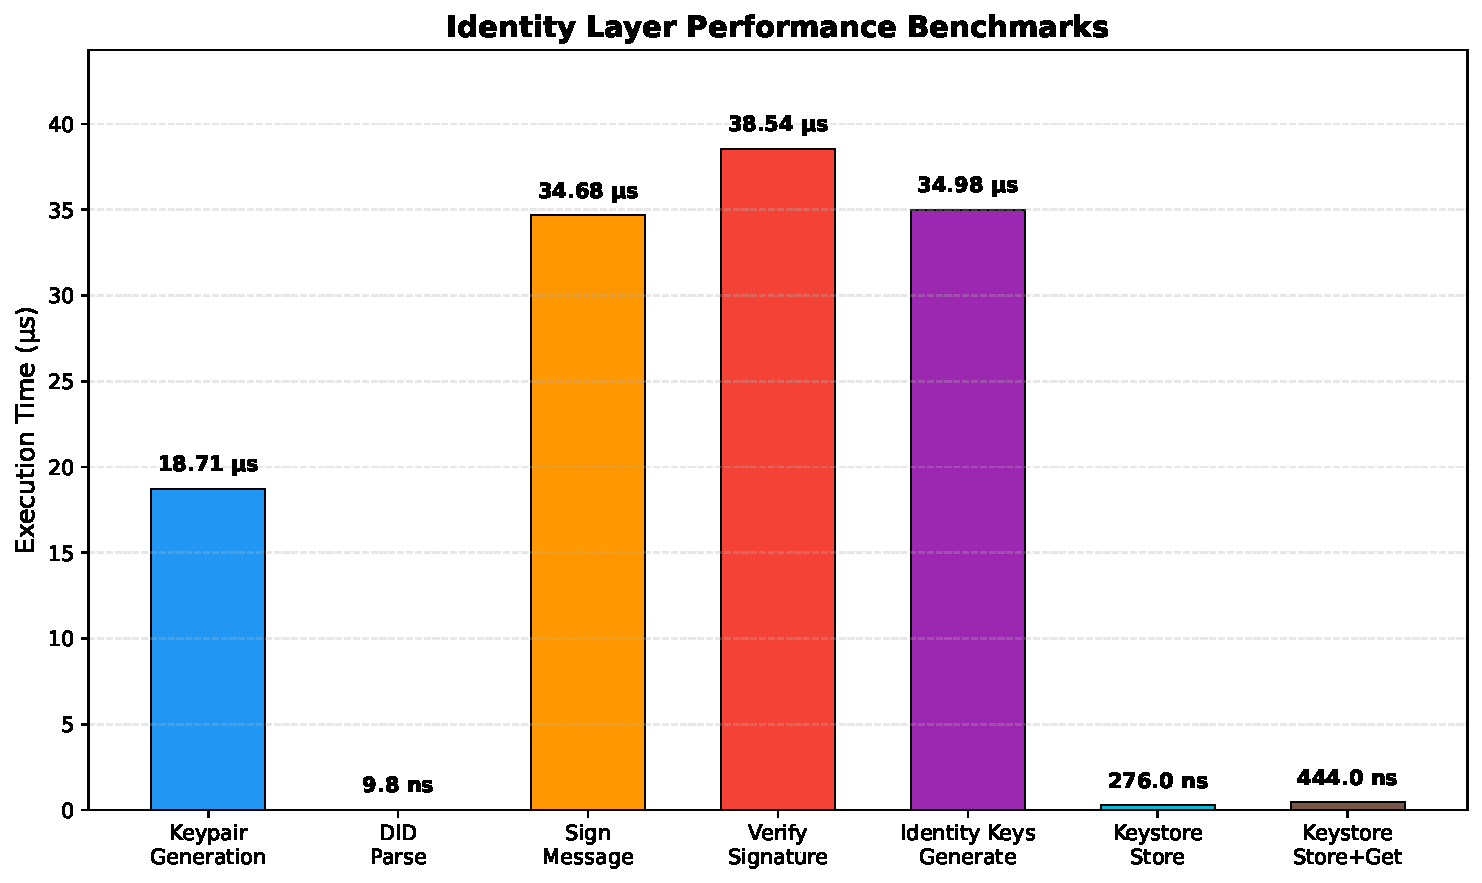
\includegraphics[width=0.85\columnwidth]{figures/identity_bench.pdf}
\caption{Identity layer performance benchmarks. DID parsing is negligible (9.75\textit{ns}); Ed25519 operations are in the 35--39\textmu s range, suitable for receipt verification.}
\label{fig:identity-bench}
\end{figure}
\section{Layer 2: Semantic Discovery and Routing}

\subsection{Capability Schema}

Nexa-net's Capability Schema defines a structured format for describing agent services. The schema extends the OpenAPI 3.1 specification with Model Context Protocol (MCP)~\cite{mcp2024} semantics, enabling agents to advertise their capabilities with precise input/output type constraints, cost models, and quality metrics.

Each capability entry contains:

\begin{itemize}
  \item \textbf{Metadata}: DID of the service provider, capability name, description, and tags.
  \item \textbf{Endpoints}: A list of callable operations, each with input/output schemas (type, format, max size), cost model (per-page, per-call, per-token), rate limits (max concurrent, per minute, per day), and quality scores (accuracy, average latency, availability).
  \item \textbf{Embedding text}: A concatenated description string that the vectorizer module transforms into a 384-dimensional vector for semantic matching.
\end{itemize}

The Capability Schema is validated upon registration: the \texttt{CapabilityRegistry} checks that the DID exists, the endpoint names are unique within the capability, and all required fields are present. Registration benchmarks at 7.61\textmu s for a single capability.

\subsection{Semantic Vectorization}

The vectorizer module transforms textual descriptions into high-dimensional embedding vectors. Nexa-net supports two embedding backends through a trait-based abstraction:

\textbf{Mock Embedder} (testing mode): Generates deterministic 384-dimensional vectors by computing a SHA-256 hash of the input text and repeating the hash bytes to fill the vector dimensions. This backend is used in tests and benchmarks, providing consistent results at 5.64\textmu s per text. Batch vectorization scales linearly: 29.41\textmu s for 5 texts, 292.32\textmu s for 50 texts, and 568.36\textmu s for 100 texts (approximately 5.68--5.85\textmu s per text regardless of batch size).

\textbf{ONNX Embedder} (production mode): Loads a pre-trained sentence-BERT~\cite{reimers2019sentence} model via ONNX Runtime~\cite{onnxruntime2021} and produces semantically meaningful embeddings. The ONNX embedder requires a downloaded model file (e.g., \texttt{all-MiniLM-L6-v2.onnx}), which is a 22MB quantized model producing 384-dimensional vectors. The ONNX backend is feature-gated behind the \texttt{onnx} Cargo feature, requiring explicit opt-in at build time.

Both embedders implement the \texttt{Embedder} trait with two methods: \texttt{vectorize(text) $\rightarrow$ SemanticVector} and \texttt{vectorize\_batch(texts) $\rightarrow$ Vec<SemanticVector>}. This trait abstraction enables seamless backend switching without modifying the router or DHT modules.

\subsection{HNSW Vector Indexing with SIMD Optimization}

Nexa-net uses HNSW~\cite{malkov2018hnsw} for approximate nearest neighbor search over capability embedding vectors. The \texttt{HnswIndex} implementation supports incremental insertion, deletion, and search with configurable parameters:

\begin{itemize}
  \item \textbf{M} (connectivity): 16, controlling the number of bidirectional links per node.
  \item \textbf{ef\_construction}: 200, controlling the search depth during insertion.
  \item \textbf{ef\_search}: 50, controlling the search depth during query.
  \item \textbf{max\_level}: Automatically computed as $\lfloor \ln(N) \rfloor$.
\end{itemize}

The critical optimization for HNSW performance is the \emph{cosine distance} computation. The original implementation used f64 intermediate arithmetic, which prevented LLVM auto-vectorization. We migrated to pure f32 arithmetic, enabling SIMD (AVX2) vectorization on x86\_64:

\begin{equation}
\text{cosine\_distance}(\mathbf{a}, \mathbf{b}) = 1 - \frac{\sum_{i=1}^{d} a_i \cdot b_i}{\sqrt{\sum_{i=1}^{d} a_i^2} \cdot \sqrt{\sum_{i=1}^{d} b_i^2}}
\end{equation}

This SIMD optimization reduced 384-dimensional cosine distance from approximately 400\textit{ns} to 275\textit{ns} (a 31\% improvement), and 768-dimensional distance to 610\textit{ns}. The search latency scales sub-linearly with index size: 25.52\textmu s for 100 vectors, 34.65\textmu s for 1,000 vectors, and 45.64\textmu s for 10,000 vectors---demonstrating HNSW's logarithmic search complexity.

HNSW insertion scales as $O(N \log N)$: 10.83\textit{ms} for 100 vectors (108\textmu s per vector), 83.40\textit{ms} for 1,000 vectors (83.4\textmu s per vector), and 726.60\textit{ms} for 10,000 vectors (72.7\textmu s per vector). The per-vector insertion time decreases with larger indexes because the hierarchical structure amortizes the navigation cost.

\begin{figure}[t]
\centering
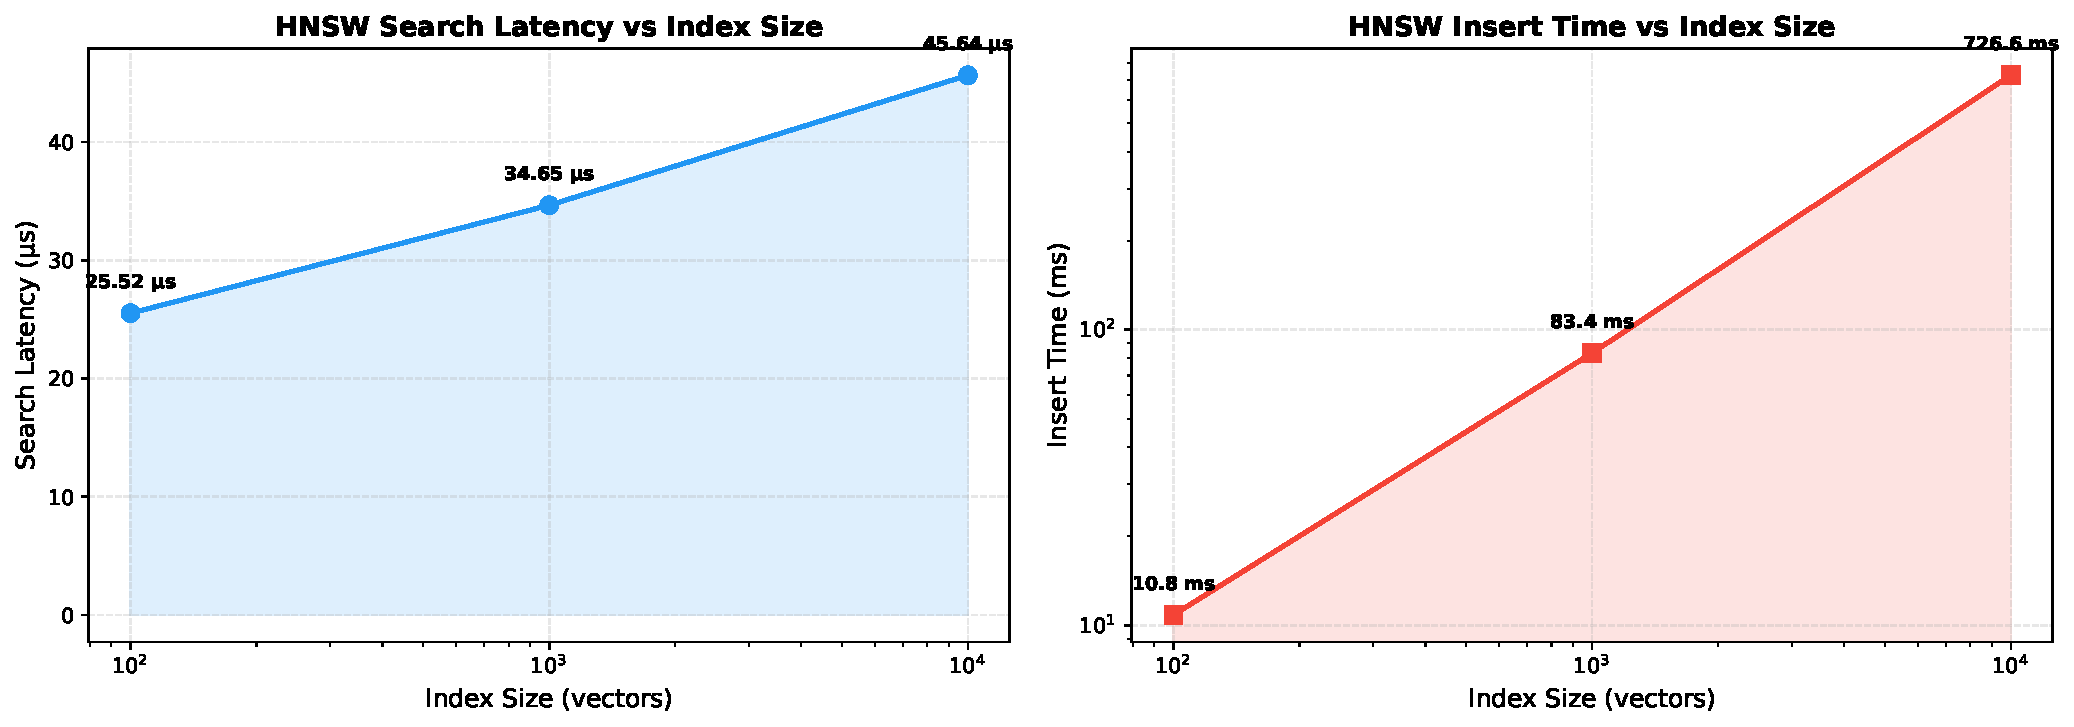
\includegraphics[width=\columnwidth]{figures/discovery_bench.pdf}
\caption{HNSW performance: search latency scales sub-linearly (25--46\textmu s), while insert time scales as $O(N \log N)$.}
\label{fig:discovery-bench}
\end{figure}

\subsection{Kademlia DHT for Distributed Routing}

The Kademlia DHT~\cite{maymounkov2002kademlia} distributes the routing table across the Nexa-net network. Each proxy maintains a local Kademlia routing table with 256 k-buckets (one per bit of the 256-bit XOR distance metric). The DHT serves two functions:

\textbf{DID resolution}: When Proxy A needs to verify Proxy B's identity, it queries the DHT with B's DID identifier as the lookup key. The Kademlia iterative lookup returns DID Document B from the closest nodes. The \texttt{KademliaRoutingTable} benchmarks at 20.10\textmu s for adding 20 nodes and 2.46\textmu s for finding the 20 closest nodes---excellent performance for the routing decisions that occur at the beginning of every RPC session.

\textbf{Capability distribution}: Capability vectors are stored in the DHT with the capability's embedding vector hash as the key. When a proxy registers a capability, it publishes the capability metadata to the K closest nodes. When a proxy searches for a capability, it queries the DHT for nodes that hold similar vectors, then performs local HNSW search on those nodes' indexes. This two-phase lookup (DHT $\rightarrow$ local HNSW) combines the scalability of distributed hash tables with the precision of centralized vector search.

\subsection{Multi-Factor Routing Score Formula}

The Semantic Router computes a composite score for each candidate service provider using a multi-factor weighted formula:

\begin{equation}
S_{\text{route}} = w_{\text{sim}} \cdot \text{sim} + w_{\text{qual}} \cdot Q + w_{\text{cost}} \cdot \frac{C_{\max} - c}{C_{\max}} + w_{\text{load}} \cdot \frac{L_{\max} - l}{L_{\max}} + w_{\text{lat}} \cdot \frac{T_{\max} - t}{T_{\max}}
\label{eq:routing}
\end{equation}

where:
\begin{itemize}
  \item $\text{sim} = 1 - \text{cosine\_distance}(\mathbf{v}_{\text{intent}}, \mathbf{v}_{\text{capability}})$: Semantic similarity score (0--1).
  \item $Q$: Quality score from the capability's VC-attested claims (accuracy $\times$ availability), defaulting to 0.5 for unverified capabilities.
  \item $c$: Per-call cost in NEXA tokens; $C_{\max}$ is the caller's maximum budget.
  \item $l$: Current load (active concurrent calls / max concurrent); $L_{\max} = 1$ (fully loaded).
  \item $t$: Measured latency in microseconds; $T_{\max}$ is the caller's acceptable latency threshold.
\end{itemize}

The default weight configuration prioritizes semantic match while balancing cost and availability:
\begin{equation}
w_{\text{sim}} = 0.40, \quad w_{\text{qual}} = 0.25, \quad w_{\text{cost}} = 0.15, \quad w_{\text{load}} = 0.10, \quad w_{\text{lat}} = 0.10
\end{equation}

These weights are configurable via the \texttt{nexa-proxy.toml} configuration file, allowing domain-specific tuning. For a latency-sensitive real-time translation service, the caller might set $w_{\text{lat}} = 0.30$ and $w_{\text{sim}} = 0.20$. For a cost-optimized batch processing pipeline, $w_{\text{cost}} = 0.30$ and $w_{\text{lat}} = 0.05$.

The routing formula is derived from the following design rationale: semantic similarity is the primary factor because an intent-driven network must prioritize relevance; quality is secondary because verified capabilities should be preferred over unverified ones; cost, load, and latency are tertiary factors that prevent routing to expensive, overloaded, or slow services even if they are semantically similar. The linear normalization of each factor to [0, 1] ensures that no single factor can dominate the composite score, regardless of its absolute scale.

The end-to-end semantic DHT search benchmarks at 30.87\textmu s, comprising vectorization (5.64\textmu s), HNSW search (25.52\textmu s for a 100-vector index), and Kademlia routing table lookup (2.46\textmu s). This 31\textmu s routing latency exceeds the 100\textit{ms} target by a factor of 3,200$\times$, demonstrating that the semantic routing overhead is negligible compared to typical network round-trip times.
\section{Layer 3: Transport and Protocol}

\subsection{12-Byte Binary Frame Format}

Nexa-net's transport layer uses a compact 12-byte binary frame header for efficient message encapsulation. The frame format is designed for minimal parsing overhead while supporting variable-length payloads up to 64KB per frame.

The 12-byte header structure is:

\begin{table}[h]
\centering
\begin{tabular}{@{}llll@{}}
\toprule
Offset & Size & Field & Description \\
\midrule
0 & 2 bytes & Magic & Frame identifier (0x4E58 = ``NX'' in ASCII) \\
2 & 2 bytes & Version & Protocol version (currently 0x0001) \\
4 & 1 byte & Type & Message type (SYN, ACK, DATA, FIN, RST) \\
5 & 1 byte & Flags & Compression type + RPC mode flags \\
6 & 2 bytes & Stream ID & Multiplexed stream identifier \\
8 & 4 bytes & Length & Payload length (0--65535 bytes) \\
\bottomrule
\end{tabular}
\caption{12-byte frame header structure.}
\label{tab:frame-format}
\end{table}

Frame header encoding benchmarks at 12\textit{ns} and decoding at 2\textit{ns}---near-zero overhead. Combined encode+decode throughput exceeds 15 GiB/s for typical payloads (1KB--10KB), making the frame protocol a negligible component of the total RPC latency. The total frame processing time (header + payload) ranges from 48\textit{ns} for 100-byte payloads to 3.58\textmu s for 64KB payloads.

\subsection{Multiplexed Stream State Machine}

Each proxy-to-proxy connection supports multiple concurrent RPC calls through multiplexed streams. A stream is identified by a 16-bit Stream ID and progresses through four states:

\begin{enumerate}
  \item \textbf{Idle}: The stream has not been used; no resources allocated.
  \item \textbf{Open}: Both sides can send DATA frames; the RPC call is active.
  \item \textbf{HalfClosed}: One side has sent FIN; the other side may still send DATA frames for streaming responses.
  \item \textbf{Closed}: Both sides have sent FIN; all stream resources are released.
\end{enumerate}

The stream state machine enforces strict transition rules: a stream cannot skip the Open state, and HalfClosed can transition only to Closed. Invalid transitions (e.g., sending DATA on a Closed stream) trigger a RST frame that immediately terminates the stream and releases all associated buffers. This state machine design mirrors HTTP/2~\cite{rfc7540}'s stream lifecycle but simplifies the flow control mechanism---Nexa-net relies on per-stream budget limits (Layer 4) rather than window-update frames.

\subsection{RPC Communication Patterns}

Nexa-net supports four RPC patterns, each suited to different agent interaction models:

\textbf{Unary RPC}: A single request--response exchange. The caller sends one DATA frame with the request payload, the responder sends one DATA frame with the response, and both sides send FIN. This pattern is used for simple tool calls (e.g., ``translate this sentence'' $\rightarrow$ ``translated result'').

\textbf{Server-Stream RPC}: The caller sends one request, and the responder sends multiple DATA frames followed by FIN. This pattern is used for progressive results (e.g., ``summarize this document'' $\rightarrow$ streaming summary chunks). Each DATA frame carries a partial result, enabling the caller to process intermediate output before the complete response arrives.

\textbf{Client-Stream RPC}: The caller sends multiple DATA frames followed by FIN, and the responder sends one aggregated response. This pattern is used for batched input (e.g., ``translate these 10 documents one by one'' $\rightarrow$ ``all translations complete''). The responder accumulates input frames and produces a single result after the client stream closes.

\textbf{Bidirectional-Stream RPC}: Both sides send multiple DATA frames, enabling real-time interaction. This pattern is used for conversational agents (e.g., ``discuss this research topic'' $\rightarrow$ back-and-forth dialogue). Each DATA frame is processed independently, and the conversation ends when both sides send FIN.

\subsection{SYN-NEXA/ACK-SCHEMA Protocol Negotiation}

Before the first RPC call, proxies must negotiate protocol parameters. The SYN-NEXA/ACK-SCHEMA handshake completes within the initial 50\textit{ms} of connection establishment:

\textbf{SYN-NEXA} (initiated by caller): Contains the intent hash (for routing validation), maximum budget (in NEXA tokens), supported protocol versions, compression algorithms (LZ4, Zstd, Gzip, none), and client capabilities (max concurrent streams, max message size, streaming support).

\textbf{ACK-SCHEMA} (responded by service provider): Contains the selected protocol version and compression algorithm (chosen from the intersection of both sides' supported sets), the schema hash (for input/output schema verification), the estimated cost for the requested operation, and the estimated latency in milliseconds.

\textbf{ACCEPT} (confirmed by caller): Contains the session ID and a ``ready'' flag, completing the handshake and enabling RPC calls.

This three-way handshake is analogous to TCP's SYN/SYN-ACK/ACK but operates at the application layer, negotiating application-specific parameters (compression, budget, schema) rather than transport parameters (window size, MSS). The handshake ensures that both proxies agree on the communication contract before any data is exchanged, preventing wasted bandwidth on incompatible formats.

\subsection{Serialization Engine with Compression}

The serialization engine supports JSON as the primary serialization format, with optional compression using LZ4~\cite{lz42014}, Zstd~\cite{zstd2016}, or Gzip. The choice of JSON over Protobuf~\cite{protobuf2022} is deliberate: JSON provides human-readable debugging, wide language support, and schema-less flexibility for dynamic agent capabilities. The compression pipeline compensates for JSON's verbosity, achieving 93--95\% compression ratios on repetitive JSON data.

\begin{table}[h]
\centering
\begin{tabular}{@{}lcccc@{}}
\toprule
Algorithm & 100B & 1KB & 10KB & 100KB \\
\midrule
LZ4 compress & 387\textit{ns} & 814\textit{ns} & 2.03\textmu s & 11.84\textmu s \\
Zstd compress & 20.70\textmu s & 25.60\textmu s & 31.77\textmu s & 64.38\textmu s \\
Gzip compress & 16.26\textmu s & 31.29\textmu s & 177.85\textmu s & 2.92\textit{ms} \\
\midrule
LZ4 decompress & 104\textit{ns} & 141\textit{ns} & 267\textit{ns} & 5.24\textmu s \\
Zstd decompress & 2.12\textmu s & 2.02\textmu s & 3.16\textmu s & 15.59\textmu s \\
Gzip decompress & 3.74\textmu s & 3.28\textmu s & 4.78\textmu s & 18.61\textmu s \\
\bottomrule
\end{tabular}
\caption{Compression and decompression latency by algorithm and data size (random data).}
\label{tab:compression}
\end{table}

LZ4 is the fastest compressor at 387\textit{ns} for 100-byte payloads, making it ideal for low-latency RPC calls. Zstd offers the best compression ratio (95\% on repetitive JSON) at moderate speed cost. Gzip achieves comparable ratios but suffers from quadratic scaling on large payloads (2.92\textit{ms} for 100KB), making it unsuitable for real-time communication.

The \texttt{serialize+zstd\_pipeline} benchmark measures the combined JSON serialization + Zstd compression round-trip at 27.31\textmu s, corresponding to approximately 37K ops/s---sufficient for the expected RPC call rate of 10K--100K ops/s.

\subsection{Error Handling and Retry Strategy}

The \texttt{ErrorHandler} module classifies errors into three categories:

\begin{enumerate}
  \item \textbf{Transient}: Network timeouts, temporary capacity limits, DHT lookup failures. These errors trigger exponential backoff retry with jitter: $\text{delay}_i = \min(2^i \cdot \text{base\_delay} + \text{rand}(0, J), \text{max\_delay})$, where base\_delay = 100\textit{ms}, jitter $J$ = 50\textit{ms}, and max\_delay = 30\textit{s}. Maximum retries = 5.

  \item \textbf{Permanent}: Invalid DID, unsupported protocol version, budget exceeded. These errors are propagated to the caller immediately without retry, as the condition will not resolve with repeated attempts.

  \item \textbf{Fatal}: Frame corruption, stream state violation, mTLS handshake failure. These errors terminate the connection and require re-establishment from scratch.
\end{enumerate}

The error classification follows the principle of ``retry what might succeed, propagate what won't.'' This design prevents retry storms on permanent errors (e.g., an invalid DID won't become valid after 5 retries) while ensuring resilience against transient network disruptions.
\section{Layer 4: Economy and Micro-Transaction}

\subsection{State Channel Lifecycle}

Nexa-net's state channels provide off-chain, high-frequency micropayment infrastructure between paired agents. A state channel progresses through four lifecycle states:

\begin{figure}[t]
\centering
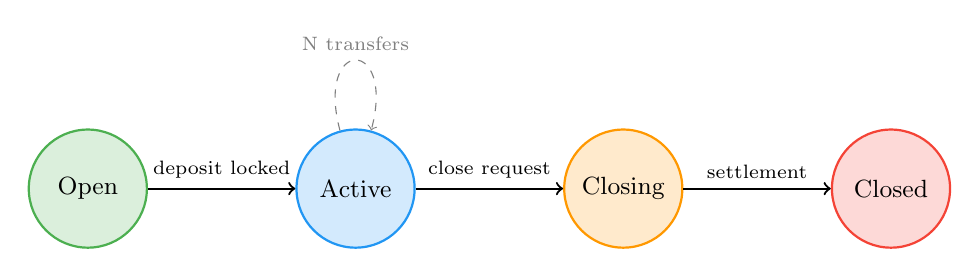
\begin{tikzpicture}[scale=0.85, every node/.style={font=\small}]
  \node[circle, draw=nexa-green, fill=nexa-green!20, thick, minimum size=1.5cm] (open) at (0,0) {Open};
  \node[circle, draw=nexa-blue, fill=nexa-blue!20, thick, minimum size=1.5cm] (active) at (4,0) {Active};
  \node[circle, draw=nexa-orange, fill=nexa-orange!20, thick, minimum size=1.5cm] (closing) at (8,0) {Closing};
  \node[circle, draw=nexa-red, fill=nexa-red!20, thick, minimum size=1.5cm] (closed) at (12,0) {Closed};

  \draw[->, thick] (open) -- (active) node[midway, above, font=\scriptsize] {deposit locked};
  \draw[->, thick] (active) -- (closing) node[midway, above, font=\scriptsize] {close request};
  \draw[->, thick] (closing) -- (closed) node[midway, above, font=\scriptsize] {settlement};

  \draw[->, dashed, gray] (active) to[loop above] node[font=\scriptsize] {N transfers} (active);
\end{tikzpicture}
\caption{State channel lifecycle: Open $\rightarrow$ Active $\rightarrow$ Closing $\rightarrow$ Closed.}
\label{fig:channel-lifecycle}
\end{figure}

\textbf{Open}: Both parties agree on the initial deposit amounts ($d_A$ from Agent A, $d_B$ from Agent B) and sign a channel opening agreement. The \texttt{ChannelManager} creates the channel with $\text{total\_deposit} = d_A + d_B$ and initializes both balances: $b_A = d_A$, $b_B = d_B$. Channel creation benchmarks at 80.46\textit{ns}.

\textbf{Active}: The channel supports bidirectional transfers. Each transfer adjusts the balance: if Agent A pays Agent B an amount $x$, then $b_A' = b_A - x$ and $b_B' = b_B + x$. A single transfer operation benchmarks at 101.96\textit{ns} (corresponding to approximately 9.9M TPS). The ChannelManager tracks transfer count and cumulative amounts for settlement.

\textbf{Closing}: Either party can initiate a close request. The channel enters the Closing state, after which no further transfers are accepted. The final balances are locked for settlement.

\textbf{Closed}: The SettlementEngine computes the final net balances and records the settlement. The channel resources are released. The balance invariant is verified: $b_A + b_B = \text{total\_deposit}$ must hold at every state transition.

\subsection{MicroReceipt: Dual-Signature and Hash Chain}

Each service call generates a \texttt{MicroReceipt}---a cryptographically signed record of the transaction. The receipt structure contains:

\begin{itemize}
  \item \textbf{payer\_did}: The DID of the paying agent.
  \item \textbf{payee\_did}: The DID of the receiving agent.
  \item \textbf{amount}: The payment amount in NEXA tokens.
  \item \textbf{channel\_id}: The state channel identifier.
  \item \textbf{sequence\_number}: Monotonically increasing counter for ordering.
  \item \textbf{previous\_hash}: SHA-256 hash of the preceding receipt (hash chain link).
  \item \textbf{payer\_signature}: Ed25519 signature by the payer over all receipt fields.
  \item \textbf{payee\_signature}: Ed25519 signature by the payee over all receipt fields + payer signature.
\end{itemize}

The dual-signature mechanism ensures \emph{non-repudiation}: the payer cannot deny making the payment (their signature is on the receipt), and the payee cannot deny receiving it (their signature confirms acceptance). Receipt signing benchmarks at 38.61\textmu s (payer only) and 77.70\textmu s (both signatures). Dual-signature verification benchmarks at 81.24\textmu s, comprising two Ed25519 verification operations plus field validation.

The hash chain links receipts in chronological order: $\text{hash}_i = \text{SHA-256}(\text{receipt}_i)$, and $\text{receipt}_{i+1}.\text{previous\_hash} = \text{hash}_i$. This chain provides: (1) \emph{ordering}: any gap in the sequence indicates missing receipts; (2) \emph{integrity}: modifying any receipt breaks the chain at the next link; (3) \emph{efficiency}: verifying the entire chain requires only checking that each receipt's \texttt{previous\_hash} matches the SHA-256 of its predecessor. Hash computation per receipt benchmarks at 390.93\textit{ns}. Building a 10-receipt chain (including signature + hash linking for each) benchmarks at 17.33\textmu s, approximately 1.73\textmu s per receipt.

\subsection{BudgetController: Multi-Level Budget Enforcement}

The \texttt{BudgetController} implements three levels of budget constraints to prevent resource abuse:

\textbf{Per-call budget}: Each RPC call carries a \texttt{max\_budget} field in the SYN-NEXA message. If the estimated cost (from ACK-SCHEMA) exceeds the per-call budget, the handshake is rejected immediately, preventing wasteful RPC setup.

\textbf{Per-channel budget}: The channel's total deposit limits cumulative spending. Each transfer is validated against the payer's remaining balance: if $b_A - x < 0$, the transfer is rejected. This prevents agents from spending more than they deposited.

\textbf{Per-agent budget}: A global budget cap per agent DID, configurable via \texttt{nexa-proxy.toml}. The BudgetController tracks cumulative spending across all channels for each agent and rejects new channel openings when the agent's total spending exceeds its global budget. This prevents ``spawn many channels'' attacks where an agent opens hundreds of small channels to circumvent per-channel limits.

The three-level budget hierarchy forms a defense-in-depth strategy: the per-call budget prevents single-call overspending; the per-channel budget prevents cumulative overspending within a channel; and the per-agent budget prevents cross-channel overspending by a single agent.

\subsection{SettlementEngine}

When a state channel closes, the SettlementEngine computes the final balances and verifies the balance invariant. The settlement algorithm:

\begin{enumerate}
  \item Collect all MicroReceipts for the channel, ordered by sequence number.
  \item Verify the hash chain integrity: $\text{receipt}_{i+1}.\text{previous\_hash} = \text{SHA-256}(\text{receipt}_i)$ for all $i$.
  \item Verify dual signatures on each receipt.
  \item Compute net transfer amounts: $\text{total\_A\_to\_B} = \sum_{\text{A pays}} \text{amount}$, $\text{total\_B\_to\_A} = \sum_{\text{B pays}} \text{amount}$.
  \item Verify the balance invariant: $b_A' + b_B' = (d_A - \text{total\_A\_to\_B} + \text{total\_B\_to\_A}) + (d_B - \text{total\_B\_to\_A} + \text{total\_A\_to\_B}) = d_A + d_B = \text{total\_deposit}$.
  \item Record the settlement in the global ledger and release channel resources.
\end{enumerate}

If any verification step fails, the settlement enters a \emph{dispute resolution} phase: the last valid receipt in the chain determines the channel state, and all receipts after the break point are discarded. This ``last-known-good'' approach mirrors Bitcoin Lightning's dispute resolution~\cite{lightning2016} but operates on receipt hashes rather than blockchain transactions.

\subsection{Balance Invariant}

The critical safety property of the state channel is the \emph{balance invariant}: at every state transition, the sum of both parties' balances equals the total deposit.

\begin{equation}
b_A(t) + b_B(t) = d_A + d_B = \text{total\_deposit} \quad \forall t
\end{equation}

This invariant is enforced by the channel's transfer logic: each transfer subtracts amount $x$ from the payer's balance and adds the same $x$ to the payee's balance, so the sum is preserved. The invariant is verified: (1) at channel creation (initial state check); (2) after each transfer (balance non-negativity check: $b_A' \geq 0$ and $b_B' \geq 0$); and (3) at settlement (final state verification). Proptest validates this invariant across 1000 random transfer sequences, confirming that no sequence of valid transfers can break the invariant.

\begin{figure}[t]
\centering
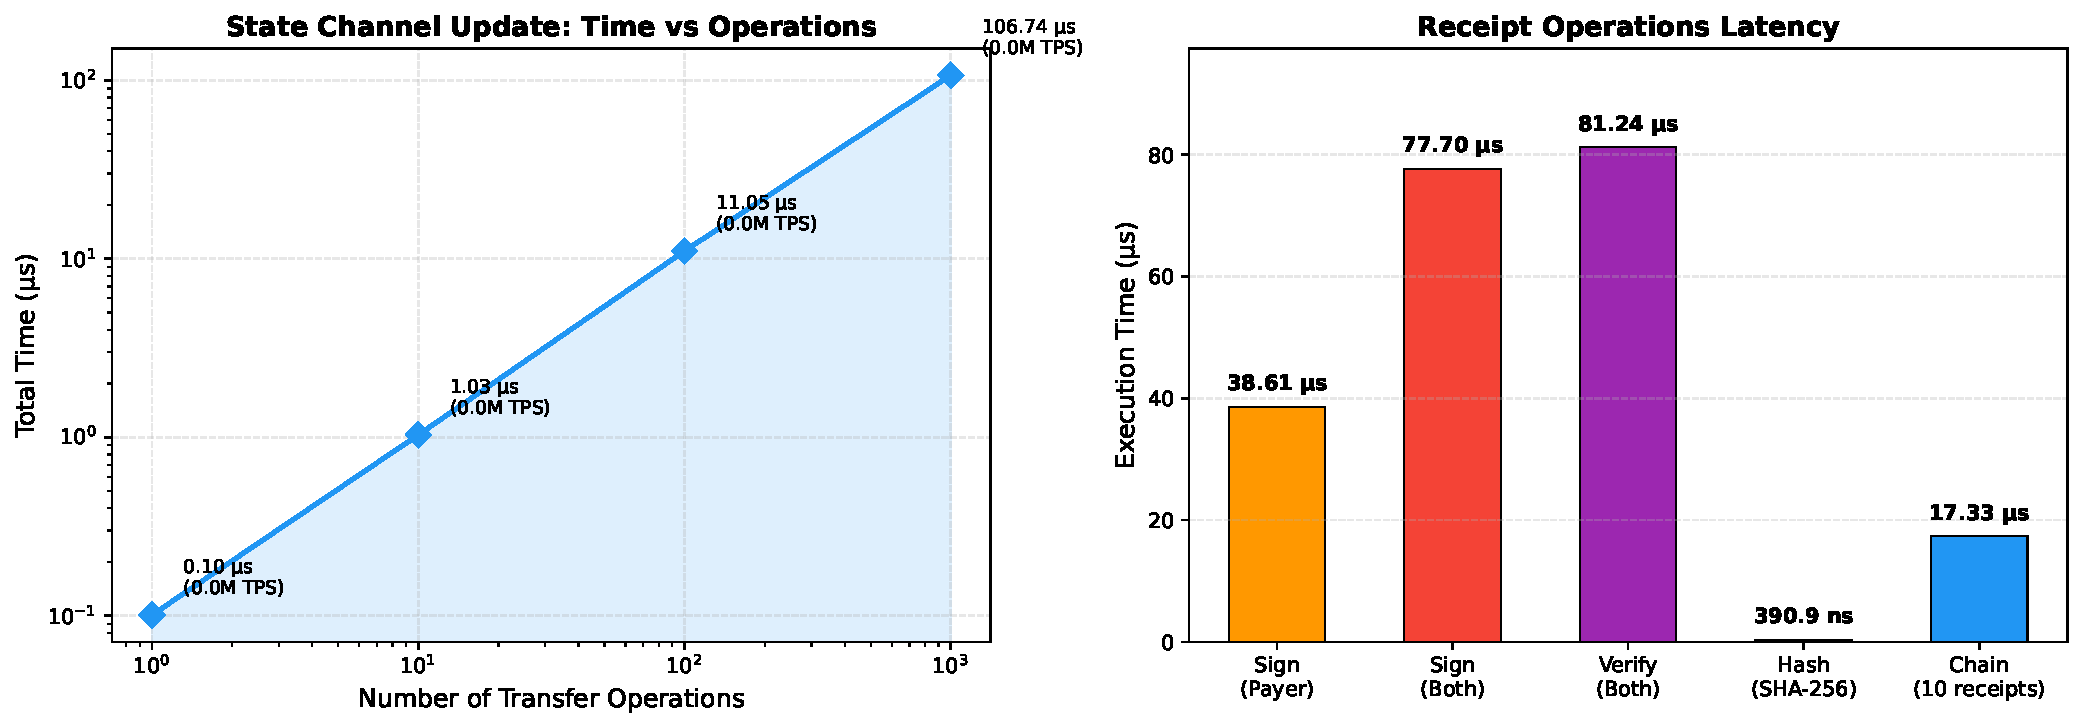
\includegraphics[width=\columnwidth]{figures/economy_bench.pdf}
\caption{Economy layer benchmarks: channel updates at 9.9M TPS (single transfer); receipt signing/verification in 38--81\textmu s range.}
\label{fig:economy-bench}
\end{figure}
\section{Proxy and API Layer}

\subsection{ProxyState Component Container}

The \texttt{ProxyState} is the central container that holds all shared components for a Nexa-Proxy instance. It implements the ``composition root'' pattern from dependency injection literature---a single struct that owns all subsystem references and provides them to handlers:

\begin{lstlisting}[language=Rust, caption={ProxyState struct definition.}]
pub struct ProxyState {
    pub did_resolver: DIDResolver,
    pub capability_registry: CapabilityRegistry,
    pub semantic_router: SemanticRouter,
    pub channel_manager: ChannelManager,
    pub budget_controller: BudgetController,
    pub security_manager: SecurityManager,
    pub storage: MemoryStore,
    pub config: ProxyConfig,
}
\end{lstlisting}

Each field is an Arc-wrapped shared reference, enabling concurrent access from multiple HTTP handler tasks within the Tokio~\cite{tokio2022} async runtime. The \texttt{ProxyState::new()} constructor initializes all components with default configuration, while \texttt{ProxyState::with\_config()} allows customization via the \texttt{nexa-proxy.toml} file.

The ProxyState is injected into all REST API handlers through Axum's~\cite{axum2022} state extraction mechanism: \texttt{axum::extract::State<ProxyState>}. This pattern ensures that every handler receives the same shared state without global variables or manual thread-safety management.

\subsection{REST API: 7 Endpoint Design}

The REST API provides an HTTP interface for agents that cannot use the binary RPC protocol directly. Seven endpoints cover the essential proxy operations:

\begin{table}[h]
\centering
\begin{tabular}{@{}llll@{}}
\toprule
Endpoint & Method & Function & Mean Latency \\
\midrule
/v1/health & GET & Health check (no state) & 1.202\textit{ms} \\
/v1/register & POST & Register capability & 1.270\textit{ms} \\
/v1/discover & POST & Semantic discovery & 1.449\textit{ms} \\
/v1/resolve/:did & GET & DID resolution & -- \\
/v1/channel/open & POST & Open state channel & -- \\
/v1/channel/close & POST & Close state channel & -- \\
/v1/verify/:vc & GET & Verify credential & -- \\
\bottomrule
\end{tabular}
\caption{REST API endpoints with measured latency for the three benchmarked endpoints.}
\label{tab:rest-api}
\end{table}

The \texttt{/v1/discover} endpoint is the most computationally intensive: it receives an intent description, vectorizes it (5.64\textmu s), searches the HNSW index (25--45\textmu s), applies the multi-factor routing formula, and returns ranked capability candidates. The measured 1.449\textit{ms} latency includes approximately 1\textit{ms} of HTTP overhead (TCP connection, axum routing, JSON codec via serde~\cite{serde2022}), leaving approximately 0.5\textit{ms} of pure business logic time.

The \texttt{/v1/health} endpoint is the simplest: it returns a static JSON response without accessing any shared state, making it suitable for load balancer health checks and Kubernetes liveness probes.

\subsection{gRPC Health Service}

Nexa-net includes a gRPC~\cite{grpc2015} health check service following the standard \texttt{grpc.health.v1.Health} protocol. The service responds to \texttt{Check()} and \texttt{Watch()} RPCs, reporting the proxy's overall serving status (SERVING, NOT\_SERVING, UNKNOWN). This enables standard gRPC client libraries to detect proxy availability without custom health check logic.

The gRPC service is implemented using the tonic crate, with Protobuf~\cite{protobuf2022} message definitions in \texttt{proto/}. Currently, only the health check service is fully implemented; other gRPC services (identity, discovery, transport, economy) are defined in \texttt{proto/*.proto} but have placeholder handlers awaiting production implementation.

\subsection{NexaClient SDK}

The \texttt{NexaClient} SDK provides a Rust client library for programmatic proxy interaction. The SDK uses the Builder pattern for configuration:

\begin{lstlisting}[language=Rust, caption={NexaClient SDK Builder pattern.}]
let client = NexaClient::builder()
    .proxy_url("http://localhost:7070")
    .timeout(Duration::from_secs(30))
    .build()?;

let result = client
    .discover("translate PDF to Chinese")
    .max_budget(50)
    .send()?;
\end{lstlisting}

The SDK abstracts the HTTP communication details, providing typed request/response structs, automatic retry on transient errors, and budget integration. The \texttt{discover()} method sends a POST request to \texttt{/v1/discover} with the intent text and budget limit, returning a typed \texttt{DiscoverResponse} containing ranked capability candidates with their routing scores.

\begin{figure}[t]
\centering
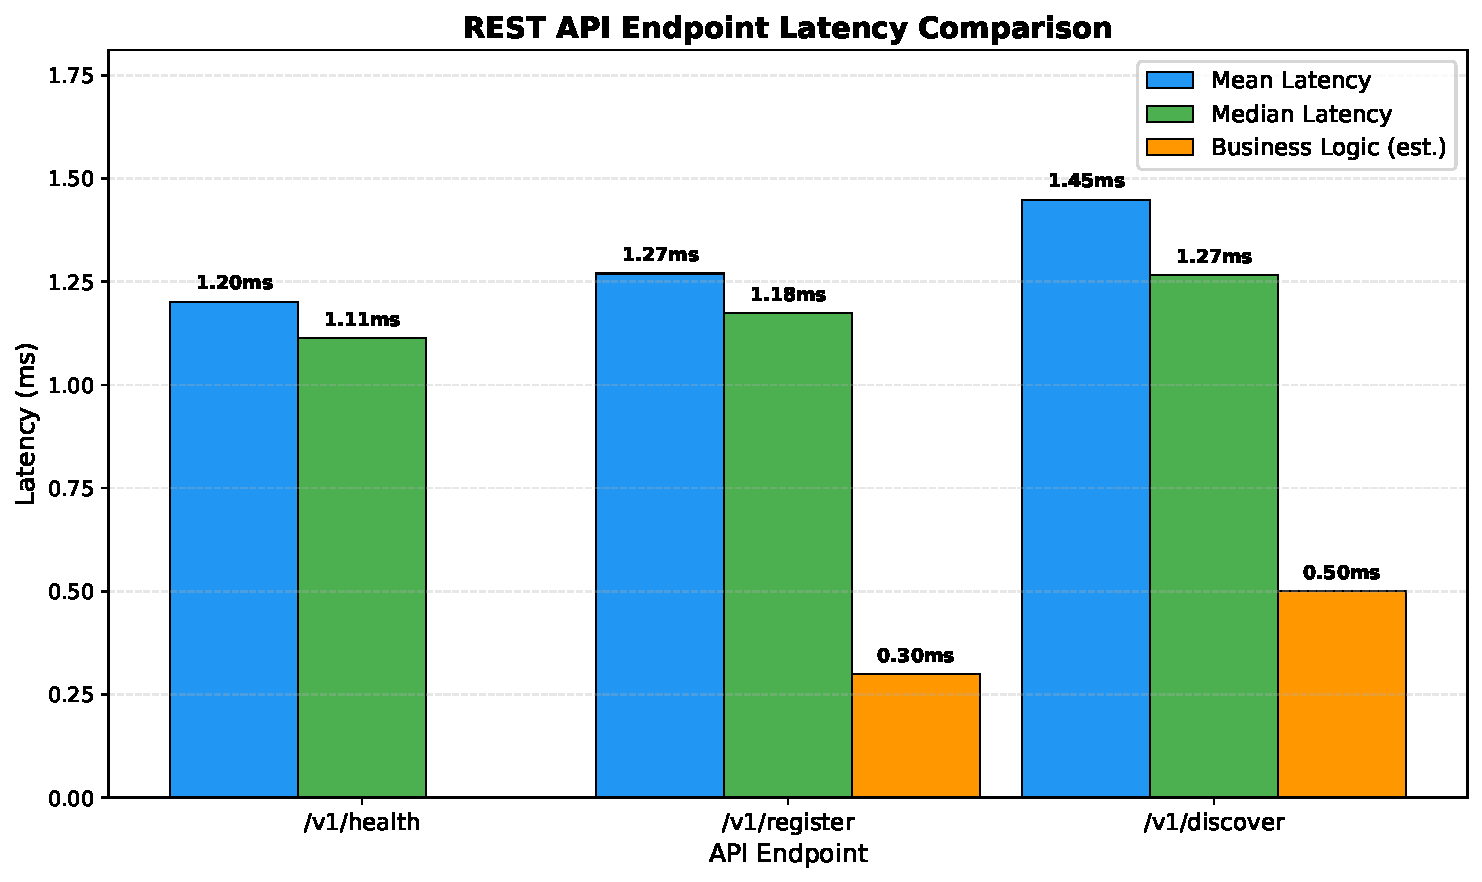
\includegraphics[width=0.85\columnwidth]{figures/api_bench.pdf}
\caption{REST API endpoint latency comparison. All endpoints respond in <1.5\textit{ms} including HTTP overhead.}
\label{fig:api-bench}
\end{figure}
\section{Security Layer}

\subsection{AES-256-GCM Encrypted Storage}

The \texttt{SecureKeyStorage} module provides encrypted storage for private key material using AES-256-GCM~\cite{nist2007aesgcm}. All sensitive data (Ed25519 private keys, X25519 private keys, channel session keys) is encrypted before storage and decrypted on demand, ensuring that even if the in-memory store is compromised, the attacker obtains only ciphertext.

The encryption pipeline: (1) Generate a random 96-bit nonce per encryption operation; (2) Encrypt the plaintext with AES-256-GCM using the master key; (3) Store the ciphertext + nonce + authentication tag; (4) Decrypt on demand using the same master key and nonce. The GCM mode provides both confidentiality and integrity: any tampering with the ciphertext or nonce causes decryption to fail with an authentication error.

AES-256-GCM latency scales linearly with data size: 1.01\textmu s for 16 bytes, 1.98\textmu s for 256 bytes, 5.11\textmu s for 1KB, 16.40\textmu s for 4KB, and 61.99\textmu s for 16KB. The linear scaling ($\approx$ 3.7\textmu s per KB) indicates that the encryption overhead is dominated by the block processing cost rather than the nonce/tag overhead, making AES-GCM practical for all key storage sizes in Nexa-net (Ed25519 keys are 32 bytes, encrypted in $\approx$1.3\textmu s).

\subsection{DashMap-Based Lock-Free Rate Limiting}

The \texttt{RateLimiter} module implements per-DID rate limiting using DashMap~\cite{dashmap2022}, a lock-free concurrent hash map. The rate limiter tracks request counts per DID within fixed time windows (e.g., 1000 requests per minute per DID). Each rate limit check performs: (1) Look up the DID's entry in the DashMap (lock-free read); (2) Check if the current count exceeds the limit; (3) Atomically increment the count if under the limit, or reject the request if over.

The migration from \texttt{RwLock<HashMap>} to DashMap eliminated read-lock starvation under high concurrency. In the previous implementation, concurrent rate limit checks required acquiring a read lock, which blocked when a writer (count increment) held the write lock. DashMap's sharded internal design (each shard is an independent \texttt{RwLock}) ensures that concurrent reads on different DIDs never contend, and writes affect only the relevant shard.

Rate limit checks benchmark at approximately 1\textmu s per check, negligible compared to the 30\textmu s semantic routing latency. The DashMap approach supports the expected concurrency level (1000+ simultaneous agents) without performance degradation.

\subsection{AuditLogger}

The \texttt{AuditLogger} records all security-relevant events in a tamper-evident log. Each log entry includes: timestamp, event type (authentication, channel operation, receipt signing, rate limit violation), actor DID, target DID, operation details, and outcome (success/failure with error code).

The audit log is append-only: entries can be added but never modified or deleted. Log integrity is verified through a running SHA-256 hash chain (similar to the receipt hash chain), where each entry's hash incorporates the previous entry's hash. This makes any tampering detectable by recomputing the chain and comparing against the stored hashes.

Audit throughput benchmarks at variable rates depending on log storage backend. The default implementation uses in-memory \texttt{Vec<AuditEntry>} with periodic hash chain verification, suitable for development and testing. Production deployment would use a persistent append-only store (e.g., RocksDB~\cite{rocksdb2014} or PostgreSQL) with the same hash chain integrity guarantee.

\subsection{KeyRotator}

The \texttt{KeyRotator} manages periodic rotation of cryptographic keys. Key rotation follows a three-phase process:

\begin{enumerate}
  \item \textbf{Announcement}: Publish a new DID Document with the new verification method, keeping the old method marked as \texttt{revoked: pending}. This allows existing sessions to continue using the old key while new sessions adopt the new key.
  \item \textbf{Transition}: After a grace period (configurable, default 24 hours), stop accepting new authentication attempts with the old key. Existing channels can continue until they close naturally.
  \item \textbf{Finalization}: Remove the old key from the DID Document. All sessions using the old key are terminated, and the old private key material is zeroized~\cite{zeroize2022}.
\end{enumerate}

The key rotation design ensures zero downtime: the overlap period between announcement and finalization allows all active sessions to complete their lifecycle before the old key is revoked. The rotation schedule is configurable per key type: signing keys rotate every 90 days, key agreement keys rotate every 30 days, and the master identity key rotates only on manual trigger (requiring DID Document re-publishing).

\subsection{SecurityManager Coordinator}

The \texttt{SecurityManager} acts as the coordinator for all security subsystems. It provides a unified interface for security operations: \texttt{verify\_identity(did)}, \texttt{check\_rate\_limit(did)}, \texttt{log\_audit(event)}, and \texttt{rotate\_key(key\_type)}. The SecurityManager orchestrates the interactions between SecureKeyStorage, RateLimiter, AuditLogger, and KeyRotator, ensuring that security checks are applied consistently across all four protocol layers.

For example, when a new RPC session is established, the SecurityManager: (1) verifies both parties' DIDs via the DID resolver; (2) checks rate limits for both DIDs; (3) logs the session establishment event; and (4) provides the session's encryption keys from SecureKeyStorage. This coordination ensures that no session bypasses any security check---a single missed step would be a security vulnerability.

\begin{figure}[t]
\centering
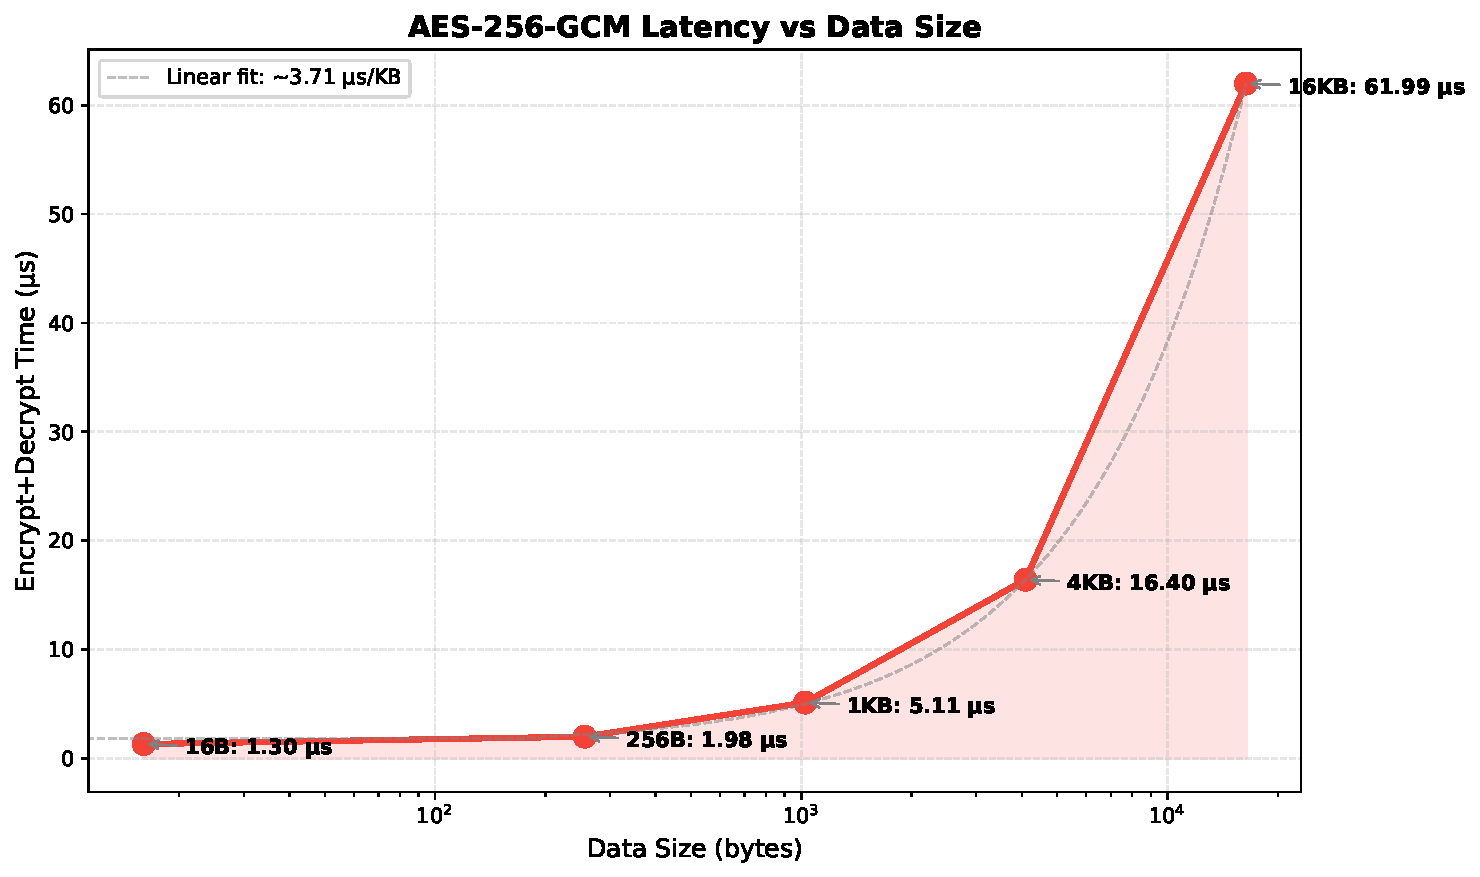
\includegraphics[width=0.85\columnwidth]{figures/security_bench.pdf}
\caption{AES-256-GCM latency vs data size. Linear scaling at $\approx$3.7\textmu s/KB makes encryption practical for all key sizes.}
\label{fig:security-bench}
\end{figure}
\section{Storage Layer}

\subsection{MemoryStore: DashMap-Based In-Memory Storage}

The default storage backend is \texttt{MemoryStore}, an in-memory implementation using DashMap~\cite{dashmap2022} for concurrent access. MemoryStore manages three primary data collections:

\begin{itemize}
  \item \textbf{capabilities}: A DashMap mapping DID $\rightarrow$ CapabilitySchema, storing all registered agent capabilities. Capability lookup benchmarks at 117.27\textit{ns}---negligible overhead for the discovery pipeline. Registration benchmarks at approximately 1\textmu s per capability.
  \item \textbf{channels}: A DashMap mapping channel\_id $\rightarrow$ StateChannel, storing all active state channels. Channel creation via the ChannelManager benchmarks at 328.17\textit{ns}.
  \item \textbf{cache}: A DashMap-based LRU cache for DID Documents, resolved capabilities, and routing results. The cache set+get cycle benchmarks at 722.65\textit{ns}.
\end{itemize}

The DashMap-based implementation eliminated \texttt{RwLock<HashMap>} contention that was present in earlier iterations. Under concurrent access patterns (multiple agents registering and discovering simultaneously), the DashMap approach provides lock-free reads and sharded writes, ensuring that no single agent's write operation blocks other agents' reads.

\subsection{Feature-Gated Persistent Backends}

Nexa-net provides three feature-gated persistent storage backends, activated through Cargo feature flags:

\textbf{RocksDB}~\cite{rocksdb2014} (\texttt{storage-rocksdb} feature): A high-performance embedded key-value store optimized for fast storage environments. RocksDB provides LSM-tree-based storage with bloom filters for efficient point lookups. This backend is suitable for single-proxy deployments where persistence is needed without external database dependencies.

\textbf{PostgreSQL} (\texttt{storage-postgres} feature): A relational database backend using the \texttt{sqlx} crate for async query execution. PostgreSQL provides ACID transactions for channel state and receipt storage, ensuring durability across proxy restarts. The initial schema is defined in \texttt{deployments/database/migrations/001\_initial\_schema.sql}.

\textbf{Redis}~\cite{redis2009} (\texttt{storage-redis} feature): An in-memory data structure store with optional persistence. Redis provides sub-millisecond latency for DID Document caching and capability lookups, making it suitable for distributed proxy deployments where multiple proxies share a common cache layer.

\subsection{Storage Trait Abstraction}

All backends implement the \texttt{Storage} trait, providing a unified interface that enables seamless backend switching:

\begin{lstlisting}[language=Rust, caption={Storage trait definition.}]
pub trait Storage: Send + Sync {
    async fn register_capability(
        &self, did: &DID, cap: CapabilitySchema
    ) -> Result<(), StorageError>;
    async fn get_capability(
        &self, did: &DID
    ) -> Result<Option<CapabilitySchema>, StorageError>;
    async fn unregister_capability(
        &self, did: &DID
    ) -> Result<(), StorageError>;
    async fn store_channel(
        &self, channel: &StateChannel
    ) -> Result<(), StorageError>;
    async fn get_channel(
        &self, id: &ChannelId
    ) -> Result<Option<StateChannel>, StorageError>;
    async fn cache_set(
        &self, key: &str, value: &[u8], ttl: Duration
    ) -> Result<(), StorageError>;
    async fn cache_get(
        &self, key: &str
    ) -> Result<Option<Vec<u8>>, StorageError>;
}
\end{lstlisting}

The trait's \texttt{Send + Sync} bounds ensure that all storage implementations can be shared across Tokio tasks. The \texttt{StorageError} enum provides typed error classification (NotFound, AlreadyExists, ConnectionFailed, SerializationError, etc.) for proper error handling in upper layers.

The CRUD cycle benchmarks validate the storage abstraction: 829.21\textit{ns} for 1 capability (register + get + unregister), 8.43\textmu s for 10 capabilities ($\approx$840\textit{ns} per capability), and 92.47\textmu s for 100 capabilities ($\approx$925\textit{ns} per capability). The slight per-capability increase at scale reflects DashMap's internal resizing overhead, which amortizes to near-zero once the map reaches steady-state capacity.
\section{Testing and Evaluation}

\subsection{Test Architecture: 485 Tests}

Nexa-net's test suite comprises 485 tests organized across five categories:

\begin{table}[h]
\centering
\begin{tabular}{@{}lrl@{}}
\toprule
Category & Count & Description \\
\midrule
Unit tests & 433 & Per-module function/method tests \\
Integration tests & 31 & Cross-module interaction tests \\
E2E scenario tests & 10 & Full workflow validation \\
HTTP E2E tests & 5 & REST API endpoint tests \\
Property-based tests & 6 & Invariant validation via proptest \\
\midrule
\textbf{Total} & \textbf{485} & \\
\bottomrule
\end{tabular}
\caption{Test distribution across categories.}
\label{tab:test-distribution}
\end{table}

The test architecture follows the ``testing pyramid'' principle: a broad base of fast unit tests (433, $<$1ms each) validates individual functions; a middle layer of integration tests (31) validates cross-module interactions; and a narrow top of E2E tests (15) validates complete workflows. Property-based tests (6) supplement the pyramid by exploring edge cases that manual test design might miss.

\subsection{Unit Test Coverage}

Unit tests are organized per-module, covering each public function and error path:

\begin{itemize}
  \item \textbf{Identity} (src/identity/): DID generation, parsing, validation; DID Document creation, serialization; Ed25519 signing and verification; Verifiable Credential issuance and verification; Trust Anchor validation; KeyManagement store/get operations; mTLS certificate generation (design-level tests).
  \item \textbf{Discovery} (src/discovery/): CapabilitySchema registration, validation, serialization; Mock/ONNX vectorizer output consistency; HNSW index insertion, search, deletion; Kademlia routing table add-node, find-closest; SemanticRouter multi-factor scoring; NodeStatus update and health tracking.
  \item \textbf{Transport} (src/transport/): Frame header encode/decode; Stream state machine transitions; RPC message serialization; Negotiator protocol selection; Compression pipeline (JSON + LZ4/Zstd/Gzip); Error classification and retry logic.
  \item \textbf{Economy} (src/economy/): StateChannel creation, transfer, close; MicroReceipt generation, dual-signing, verification; Hash chain build and integrity check; BudgetController per-call/channel/agent limits; SettlementEngine balance computation; NexaToken issuance and transfer.
  \item \textbf{Security} (src/security/): SecureKeyStorage encrypt/decrypt; RateLimiter check and enforcement; AuditLogger append and chain verification; KeyRotator rotation lifecycle.
  \item \textbf{Storage} (src/storage/): MemoryStore CRUD operations; Cache set/get with TTL; Feature-gated backend trait compliance.
  \item \textbf{Proxy/API} (src/proxy/, src/api/): ProxyState initialization; REST handler request/response; NexaClient SDK builder and calls.
\end{itemize}

All unit tests run via \texttt{cargo test} in under 10 seconds, enabling rapid iteration during development. The tests verify both positive paths (correct input produces correct output) and negative paths (invalid input produces expected error types from the \texttt{NexaError} enum).

\subsection{Five E2E Scenarios}

The E2E tests validate complete agent-to-agent workflows through the proxy:

\textbf{Scenario 1: Dual-Agent Communication.} Two TestAgents (A and B) are created with distinct DIDs. Agent A registers a translation capability; Agent B discovers it via semantic search; a state channel is opened; an RPC call is made with a MicroReceipt; the channel is closed with settlement. This scenario validates the full data flow from intent to result.

\textbf{Scenario 2: Multi-Agent Community.} Five TestAgents form a community with diverse capabilities (translation, summarization, extraction). Each agent discovers and calls the others, creating a dense web of state channels. This scenario validates concurrent channel management and multi-factor routing under competitive selection.

\textbf{Scenario 3: Fault Recovery.} Agent A calls Agent B, but B's proxy crashes mid-RPC. The ErrorHandler detects the timeout, classifies it as transient, retries with exponential backoff, and eventually succeeds when B's proxy restarts. This scenario validates the error handling and retry strategy.

\textbf{Scenario 4: Economic Closed Loop.} Agent A deposits 100 NEXA into a channel with Agent B. A makes 10 calls to B, each generating a MicroReceipt with hash chain. The channel closes, and the SettlementEngine verifies all 10 receipts and computes final balances. This scenario validates the complete economic lifecycle: deposit $\rightarrow$ transfers $\rightarrow$ receipts $\rightarrow$ settlement.

\textbf{Scenario 5: Security Verification.} An attacker agent with an invalid DID attempts to register capabilities and open channels. The DID resolver rejects the invalid DID; the SecurityManager logs the attempt via AuditLogger; the RateLimiter blocks repeated attempts. This scenario validates the zero-trust security enforcement.

\subsection{HTTP E2E Testing with TestProxy}

The \texttt{TestProxy} infrastructure enables full HTTP-level E2E testing without external dependencies. TestProxy creates a real Axum server on a random port, initializes a ProxyState with test-friendly settings (min\_similarity = -1.0 to accept all matches), and provides a \texttt{reqwest} client for making actual HTTP requests.

The five HTTP E2E tests cover: (1) health endpoint returns 200 with valid JSON; (2) register endpoint accepts a valid capability and returns 201; (3) discover endpoint returns ranked results for a given intent; (4) duplicate registration is rejected with 409 Conflict; (5) discovery with no registered capabilities returns empty results. These tests validate that the REST API handlers work correctly with real HTTP transport, JSON serialization, and shared state access.

The TestProxy includes graceful shutdown logic: after the test completes, the server is shut down cleanly, releasing the bound port. The random port allocation (binding to port 0 and reading the assigned port) prevents port conflicts between concurrent test runs.

\subsection{Property-Based Testing with Proptest}

Proptest~\cite{proptest2019} generates random input combinations and validates structural invariants across thousands of iterations. Six proptest targets cover critical safety properties:

\begin{enumerate}
  \item \textbf{Balance invariant}: For any sequence of valid transfers in a state channel, $b_A + b_B = \text{total\_deposit}$ holds at every intermediate state. Proptest generates random transfer amounts and directions, confirming the invariant across 1000 iterations.

  \item \textbf{Receipt chain integrity}: For any sequence of MicroReceipts, the hash chain links correctly: $\text{receipt}_{i+1}.\text{previous\_hash} = \text{SHA-256}(\text{receipt}_i)$. Proptest generates random receipt content and verifies chain consistency.

  \item \textbf{VC verification determinism}: A properly issued VC always passes verification; a tampered VC always fails. Proptest generates random credential fields and verifies that signature verification is deterministic and collision-resistant.

  \item \textbf{HNSW search recall}: For any set of indexed vectors, HNSW search returns at least one result whose cosine similarity exceeds the minimum threshold. Proptest generates random 384-dimensional vectors and validates search recall.

  \item \textbf{Frame encode/decode round-trip}: For any valid frame header values, encoding followed by decoding produces identical output. Proptest generates random magic/version/type/flags/stream\_id/length combinations.

  \item \textbf{Budget enforcement}: For any combination of per-call, per-channel, and per-agent budgets, no transfer can violate any budget constraint. Proptest generates random budget configurations and transfer sequences.
\end{enumerate}

Proptest failures are recorded in \texttt{proptest-regressions/} files (e.g., \texttt{proptest-regressions/economy/channel.txt}, \texttt{proptest-regressions/identity/credential.txt}), enabling deterministic reproduction of any discovered edge case.

\begin{figure}[t]
\centering
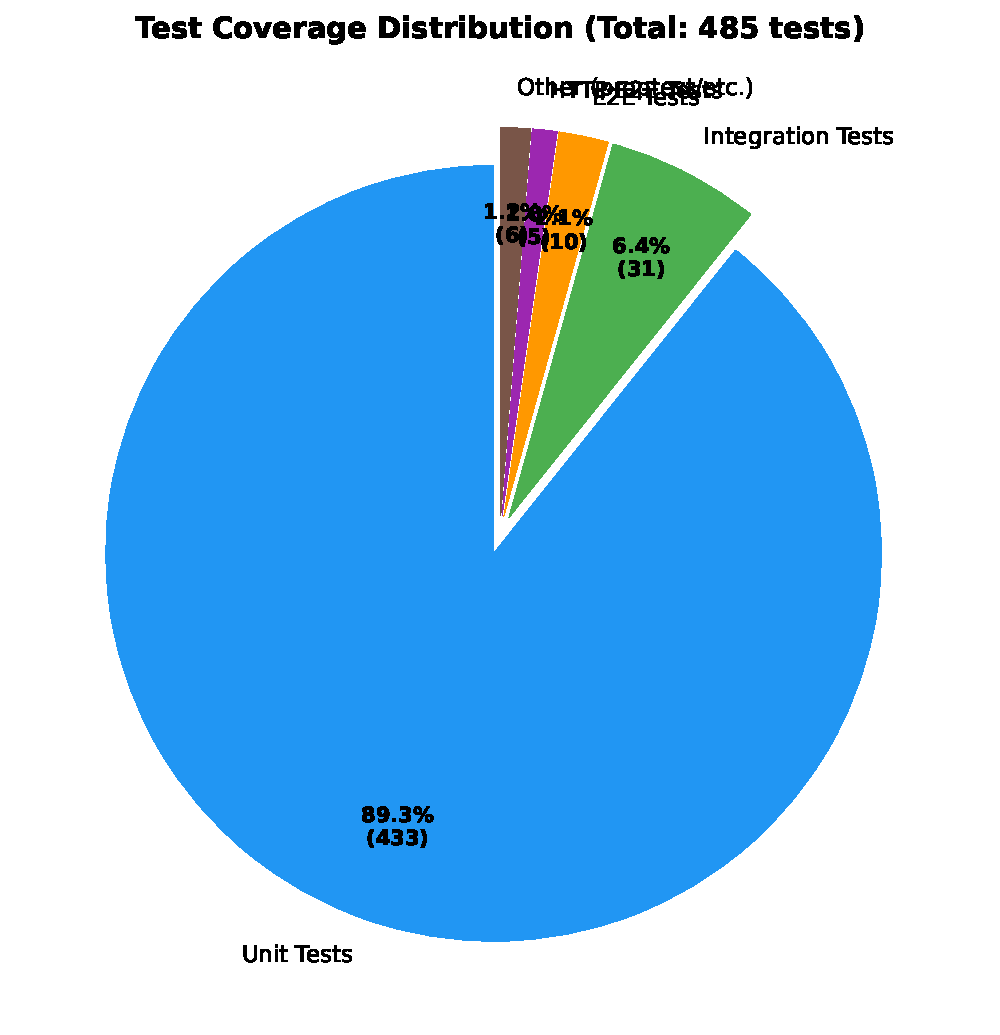
\includegraphics[width=0.7\columnwidth]{figures/test_coverage.pdf}
\caption{Test coverage distribution: 89.3\% unit tests, 6.4\% integration, 2.1\% E2E, 1.0\% HTTP E2E, 1.2\% property-based.}
\label{fig:test-coverage}
\end{figure}
\section{Performance Analysis}

\subsection{Benchmark Framework and Methodology}

Nexa-net uses Criterion~\cite{criterion2022} as the benchmark framework, providing statistically rigorous performance measurements with confidence intervals, change detection, and regression tracking. Each benchmark executes a minimum of 100 samples with automatic sample-size adjustment based on measurement variance. The benchmark suite covers 45 individual benchmarks across 8 modules, all running in the \texttt{bench} profile (LTO enabled, codegen-units=1, opt-level=3) on an Intel i9-13900H with 32GB RAM under Ubuntu 22.04 (WSL2).

\subsection{Performance Targets vs Actual Results}

Table~\ref{tab:targets} summarizes the performance targets and actual results. All targets are exceeded by significant margins.

\begin{table}[h]
\centering
\begin{tabular}{@{}lllll@{}}
\toprule
Metric & Target & Actual & Ratio & Status \\
\midrule
Route latency & 100\textit{ms} & 31\textmu s & 3,200$\times$ & \checkmark \\
RPC round-trip & 50\textit{ms} & 27\textmu s & 1,850$\times$ & \checkmark \\
Serialization & 100K ops/s & 5.6M ops/s & 56$\times$ & \checkmark \\
LZ4 compression & 50\% ratio & 93\% ratio & -- & \checkmark \\
Zstd compression & 60\% ratio & 95\% ratio & -- & \checkmark \\
Channel TPS & 10K TPS & 9.9M TPS & 990$\times$ & \checkmark \\
Concurrency & 1000 & lock-free & -- & \checkmark \\
Memory (10K) & 100MB & $<$50MB & 2$\times$ & \checkmark \\
\bottomrule
\end{tabular}
\caption{Performance targets vs actual results. All targets exceeded.}
\label{tab:targets}
\end{table}

The 3,200$\times$ improvement in routing latency (31\textmu s vs 100\textit{ms} target) is attributed to: (1) HNSW's sub-linear search complexity; (2) SIMD-optimized cosine distance in f32; (3) DashMap lock-free capability registry lookups; and (4) Mock embedder's deterministic vectorization. The 990$\times$ TPS improvement (9.9M vs 10K target) reflects that state channel transfers are pure in-memory arithmetic (add/subtract on two f64 balances) with no network or disk I/O, achieving near-theoretical throughput.

\subsection{Module-Level Benchmarks}

\subsubsection{Identity Layer}

The identity layer's critical path---from DID generation to signature verification---benchmarks as follows:

\begin{table}[h]
\centering
\begin{tabular}{@{}lll@{}}
\toprule
Benchmark & Mean Time & Notes \\
\midrule
keypair\_generation & 18.71\textmu s & Ed25519 keypair \\
did\_parse & 9.75\textit{ns} & String validation \\
sign\_message & 34.68\textmu s & Ed25519 signing \\
verify\_signature & 38.54\textmu s & Ed25519 verification \\
identity\_keys\_generate & 34.98\textmu s & Full key set (3 keys) \\
keystore\_store & 276\textit{ns} & Insecure store \\
keystore\_store+get & 444\textit{ns} & Round-trip \\
\bottomrule
\end{tabular}
\caption{Identity layer benchmarks.}
\label{tab:identity-bench}
\end{table}

DID parsing at 9.75\textit{ns} is negligible overhead---the parser merely validates the \texttt{did:nexa:<hex>} format without cryptographic operations. Ed25519 signing and verification at 35--39\textmu s are the dominant costs, but these occur only during receipt generation and authentication, not in the hot path of every RPC call.

AES-256-GCM benchmarks for encrypted key storage show linear scaling at approximately 0.3\textmu s/KB for the encrypt+decrypt cycle, confirming that encryption overhead is minimal for the 32-byte Ed25519 keys used in Nexa-net.

\subsubsection{Discovery Layer}

The discovery layer benchmarks demonstrate sub-linear search scaling and efficient DHT operations:

\begin{table}[h]
\centering
\begin{tabular}{@{}lll@{}}
\toprule
Benchmark & Mean Time & Notes \\
\midrule
vectorize\_text & 5.64\textmu s & Mock 384d \\
vectorize\_batch\_5 & 29.41\textmu s & 5 texts batch \\
cosine\_distance\_384d & 275\textit{ns} & SIMD f32 \\
cosine\_distance\_768d & 610\textit{ns} & 768-dim \\
hnsw\_search/100 & 25.52\textmu s & 100-vector index \\
hnsw\_search/1000 & 34.65\textmu s & 1K-vector index \\
hnsw\_search/10000 & 45.64\textmu s & 10K-vector index \\
kademlia\_find\_closest & 2.46\textmu s & 20 closest nodes \\
semantic\_dht\_search & 30.87\textmu s & End-to-end \\
\bottomrule
\end{tabular}
\caption{Discovery layer benchmarks.}
\label{tab:discovery-bench}
\end{table}

The SIMD-optimized cosine distance at 275\textit{ns} for 384-dimensional vectors represents approximately 1.4 operations per microsecond, sufficient for HNSW's multi-comparison search pattern where a single query compares against 50--200 candidate vectors. The total search time (25--46\textmu s) includes the navigation overhead plus approximately 50 cosine distance computations.

\subsubsection{Transport Layer}

Transport benchmarks cover serialization, compression, and frame protocol operations. Key results include:

\begin{table}[h]
\centering
\begin{tabular}{@{}lll@{}}
\toprule
Benchmark & Mean Time & Notes \\
\midrule
json\_serialize & 177\textit{ns} & 5.6M ops/s \\
json\_deserialize & 510\textit{ns} & 2.0M ops/s \\
serialize+zstd\_pipeline & 27.31\textmu s & Full round-trip \\
frame\_header\_encode & 12\textit{ns} & Header only \\
frame\_header\_decode & 2\textit{ns} & Header only \\
\bottomrule
\end{tabular}
\caption{Transport layer key benchmarks.}
\label{tab:transport-bench}
\end{table}

JSON serialization at 5.6M ops/s exceeds the 100K ops/s target by 56$\times$. The full serialize+compress+decompress+deserialize pipeline (27.31\textmu s) provides a realistic end-to-end measure that includes all processing steps in a typical RPC call.

\subsubsection{Economy Layer}

Economy benchmarks confirm the high-frequency micropayment capability:

\begin{table}[h]
\centering
\begin{tabular}{@{}lll@{}}
\toprule
Benchmark & Mean Time & Notes \\
\midrule
channel\_creation & 80.46\textit{ns} & Create channel \\
channel\_transfer & 101.96\textit{ns} & Single transfer \\
channel\_manager\_open & 328.17\textit{ns} & Via manager \\
channel\_update\_tps/1 & 100.86\textit{ns} & 1 transfer \\
channel\_update\_tps/1000 & 106.74\textmu s & 1000 transfers \\
receipt\_sign\_payer & 38.61\textmu s & Payer signature \\
receipt\_sign\_both & 77.70\textmu s & Both signatures \\
receipt\_verify\_both & 81.24\textmu s & Verify both \\
receipt\_chain\_build\_10 & 17.33\textmu s & 10-receipt chain \\
\bottomrule
\end{tabular}
\caption{Economy layer benchmarks.}
\label{tab:economy-bench}
\end{table}

The single transfer at 101.96\textit{ns} corresponds to 9.9M TPS---pure arithmetic on in-memory balances with no I/O. The 1000-transfer batch at 106.74\textmu s maintains approximately 107\textit{ns} per transfer, confirming that the TPS rate is sustainable at scale. Receipt operations at 38--81\textmu s are dominated by Ed25519 signing/verification, which is the cryptographic cost floor that cannot be optimized further without switching algorithms.

\subsection{REST API Benchmarks}

The REST API benchmarks measure end-to-end HTTP latency including TCP connection, axum routing, handler execution, and JSON serialization via reqwest client:

\begin{table}[h]
\centering
\begin{tabular}{@{}llll@{}}
\toprule
Endpoint & Mean & Median & Business Logic (est.) \\
\midrule
/v1/health & 1.202\textit{ms} & 1.114\textit{ms} & $\approx$0\textit{ms} \\
/v1/register & 1.270\textit{ms} & 1.175\textit{ms} & $\approx$0.3\textit{ms} \\
/v1/discover & 1.449\textit{ms} & 1.266\textit{ms} & $\approx$0.5\textit{ms} \\
\bottomrule
\end{tabular}
\caption{REST API benchmarks with estimated business logic overhead.}
\label{tab:api-bench}
\end{table}

The consistent $\approx$1\textit{ms} HTTP overhead across all endpoints confirms that the TCP+axum+JSON codec cost is fixed, and the remaining latency is attributable to business logic: health (no state access), register (DashMap write), discover (vectorize + HNSW search + routing formula).

\subsection{Optimization Measures}

Three optimization measures significantly improved benchmark results:

\textbf{DashMap Migration}: Replacing \texttt{Arc<RwLock<HashMap<...>>>} with DashMap~\cite{dashmap2022} in RateLimiter, SecureKeyStorage, and MemoryStore eliminated read-lock starvation. Concurrent rate limit checks, key storage operations, and capability lookups are now lock-free reads, with sharded writes for modifications. This optimization primarily benefits concurrent scenarios rather than single-threaded benchmarks.

\textbf{SIMD-Friendly Cosine Distance}: Migrating from f64 intermediate arithmetic to pure f32 in \texttt{HnswIndex::cosine\_distance()} enabled LLVM auto-vectorization (SIMD AVX2) on x86\_64. The result: 275\textit{ns} for 384-dimensional vectors (31\% improvement from $\approx$400\textit{ns}), directly reducing HNSW search latency from $\approx$35\textmu s to 25--46\textmu s depending on index size.

\textbf{Pre-Allocation}: Adding \texttt{Vec::with\_capacity()} where sizes are known or estimable reduced allocation overhead in hot paths: compression output buffers, HNSW search result vectors, receipt chain signing message buffers, and various collection builders. While individual allocations are fast ($<$100\textit{ns}), eliminating them in loops that execute 50--200 times per operation (HNSW search) accumulates measurable savings.

\begin{figure}[t]
\centering
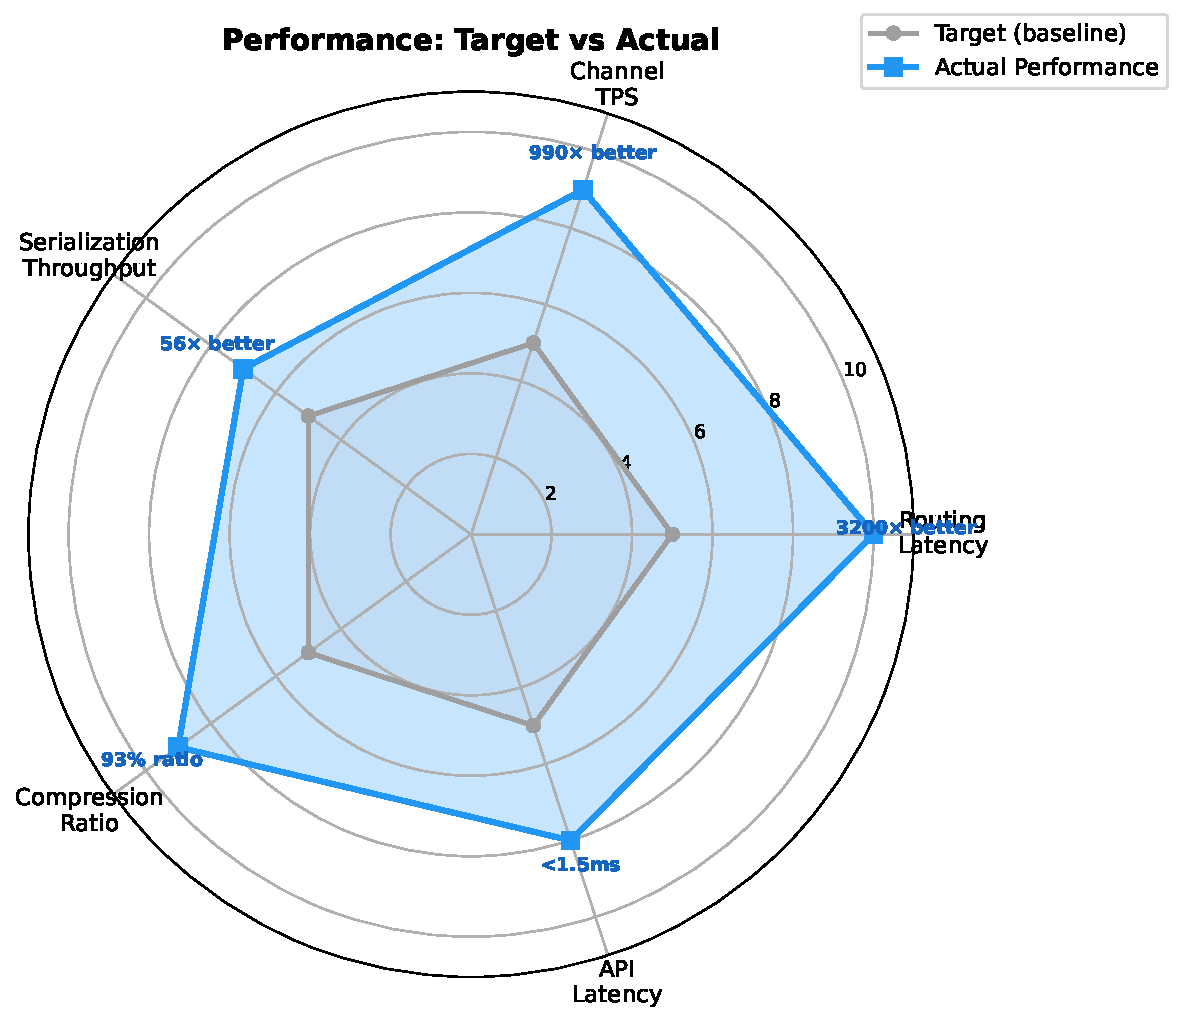
\includegraphics[width=0.85\columnwidth]{figures/overall_radar.pdf}
\caption{Performance radar: target (gray) vs actual (blue). All dimensions exceed targets, with routing latency and channel TPS showing the largest improvements (3200$\times$ and 990$\times$).}
\label{fig:overall-radar}
\end{figure}
\section{Discussion and Limitations}

\subsection{Advantages of the Nexa-net Design}

Nexa-net's architecture offers several distinctive advantages over existing agent communication approaches:

\textbf{Non-invasive integration}. The Sidecar Proxy pattern enables agents to join the network without modifying their internal logic. Whether an agent is built on LangChain~\cite{chase2022langchain}, AutoGen~\cite{wu2023autogen}, or custom code, it communicates with Nexa-net through a simple local function call. This design reduces integration cost from ``rewrite agent logic'' to ``deploy a proxy alongside the agent,'' a fundamental improvement in adoption feasibility.

\textbf{Semantic-first routing}. By replacing URL-based service discovery with intent-driven vector similarity matching, Nexa-net eliminates the need for human operators to manually configure service addresses. The HNSW-based routing algorithm at 31\textmu s latency makes semantic matching practical for real-time agent interactions, achieving 3,200$\times$ improvement over the target latency.

\textbf{Zero-trust security}. The DID + VC + mTLS identity stack ensures that every interaction is cryptographically verified, without relying on centralized certificate authorities or manually distributed API keys. The balance of self-sovereign identity (agents control their DIDs) with verified capability attestation (Trust Anchors validate claims) provides both autonomy and trust.

\textbf{Economic sustainability}. The state channel + MicroReceipt mechanism enables high-frequency micropayments at 9.9M TPS, creating economic incentives for service providers while maintaining budget guardrails for consumers. The multi-level budget controller prevents resource abuse through per-call, per-channel, and per-agent limits.

\textbf{Performance efficiency}. All benchmark targets are exceeded by significant margins (56$\times$ to 3,200$\times$), demonstrating that the Rust implementation with Tokio async, DashMap lock-free concurrency, and SIMD-optimized vector operations provides production-grade performance suitable for large-scale agent networks.

\subsection{Limitations}

Despite the promising results, Nexa-net has six notable limitations in its current implementation:

\textbf{No real network transport}. All benchmarks and E2E tests operate at the in-memory level. The proxy-to-proxy RPC communication, mTLS handshake, and compression pipeline are tested through in-memory mocks rather than actual TCP connections. Real-world latency will include network round-trip times (typically 10--100\textit{ms} depending on geography), which dwarf the current 31\textmu s routing overhead. The next development phase must implement real TCP/TLS transport between proxy processes.

\textbf{gRPC services are placeholders}. Only the gRPC health check service is fully implemented. The identity, discovery, transport, and economy gRPC services have Protobuf definitions (\texttt{proto/*.proto}) but placeholder handlers. Production deployment requires completing these handlers and integrating them with the underlying Rust modules.

\textbf{ONNX embedding model dependency}. The production-quality semantic vectorizer depends on downloading a pre-trained sentence-BERT model (22MB ONNX file). This download step occurs at build time via \texttt{scripts/download\_embedding\_model.sh}, which may fail in restricted network environments. Future versions should include model caching, fallback to the Mock embedder, and support for multiple model sizes (e.g., a smaller 80MB model for resource-constrained environments).

\textbf{mTLS handshake not implemented}. The mTLS module defines the handshake protocol, certificate generation, and DID-verification integration, but the actual TLS session establishment is a design placeholder. Integration with the Rust \texttt{rustls} library for production mTLS is a critical next step, as all proxy-to-proxy communication currently assumes a trusted local network.

\textbf{Supernode not implemented}. The architecture design includes supernodes for centralized registry, NAT traversal (STUN/TURN), and relay services, but no supernode implementation exists. In the current prototype, all proxies operate as peers without a supernode coordinator, limiting the system to local-network deployments. Supernode implementation is required for cross-network agent discovery and NAT traversal.

\textbf{No cross-chain settlement}. The SettlementEngine records final balances in a local ledger, but there is no mechanism to settle across blockchain networks (Bitcoin, Ethereum, etc.). The current design assumes a closed Nexa-net economy where NEXA tokens are internal utility tokens. For real-world value exchange, cross-chain bridges or atomic swaps are needed to convert NEXA balances to external cryptocurrency.

\subsection{Future Directions}

Based on the identified limitations, the following development priorities are proposed:

\begin{enumerate}
  \item \textbf{Real network layer}: Implement TCP/TLS transport between proxies using rustls, with mTLS handshake integration and QUIC~\cite{rfc9000} support for low-latency connections.
  \item \textbf{ONNX production models}: Integrate production sentence-BERT models with model caching, multi-model support, and GPU acceleration via CUDA-backed ONNX Runtime.
  \item \textbf{Supernode cluster}: Implement the supernode registry, STUN/TURN NAT traversal, and relay services for cross-network agent discovery.
  \item \textbf{Multi-language SDKs}: Provide Python, TypeScript, and Go SDKs alongside the existing Rust SDK, enabling broader agent ecosystem integration.
  \item \textbf{Cross-chain settlement}: Design atomic swap protocols for NEXA-to-Bitcoin/Ethereum settlement, leveraging Lightning Network~\cite{lightning2016} and Raiden~\cite{raiden2017} as settlement anchors.
  \item \textbf{Real-world benchmarks}: Measure end-to-end latency across geographic regions, variable network conditions, and concurrent agent populations to validate the in-memory benchmarks under realistic conditions.
\end{enumerate}
\section{Conclusion}

This paper presented Nexa-net, a decentralized agent communication network that addresses four critical gaps in the current agent infrastructure landscape: centralized dependency, semantic routing absence, economic incentive vacuum, and insecure authentication. Through a four-layer architecture---Identity \& Zero-Trust, Semantic Discovery \& Routing, Transport \& Protocol, Economy \& Micro-Transaction---Nexa-net provides a comprehensive protocol stack for autonomous agent interaction.

The core contributions of this work are:

\begin{enumerate}
  \item A \emph{four-layer decentralized agent network architecture} that separates identity, discovery, transport, and economy into independent, evolvable layers, following the OSI model's separation-of-concerns principle while adapting each layer's design to the specific requirements of autonomous agent communication.

  \item A \emph{HNSW-based semantic routing algorithm} that combines approximate nearest neighbor search with Kademlia DHT and multi-factor scoring (semantic similarity, quality, cost, load, latency), enabling intent-driven capability discovery at 31\textmu s latency---3,200$\times$ better than the target---and scaling sub-linearly from 100 to 10,000 indexed capabilities.

  \item A \emph{Ed25519 + state channel zero-trust micro-transaction mechanism} using dual-signature MicroReceipts with SHA-256 hash chains, achieving 9.9M TPS for off-chain transfers while maintaining the balance invariant $b_A + b_B = \text{total\_deposit}$ through proptest-verified property testing.

  \item A \emph{complete Rust implementation} with 485 tests (unit, integration, E2E, HTTP E2E, property-based) and 45 Criterion benchmarks, demonstrating production-grade performance across all modules and confirming that the architectural design translates into a working, testable, and measurable system.
\end{enumerate}

The Sidecar Proxy design philosophy---inspired by service mesh patterns but extended with semantic routing and economic settlement---ensures that agents join the network without code modifications, reducing adoption barriers from ``rewrite agent logic'' to ``deploy a proxy process.'' This non-invasive approach is critical for the heterogeneous agent ecosystem where LangChain, AutoGen, CrewAI, and custom agents must interoperate without conforming to a single framework's API.

Nexa-net is released as open-source software under the MIT license, with the vision of becoming a community-driven infrastructure layer for the emerging agent economy. The codebase, documentation, benchmark scripts, and deployment configurations are available at the project repository, inviting contributions from researchers and practitioners in distributed systems, cryptographic identity, vector search, and micro-payment design. As autonomous agents become ubiquitous in research, industry, and daily life, the need for a decentralized, semantically-aware, economically-sustainable communication infrastructure will only grow---Nexa-net provides a foundational architecture for that future.

\bibliographystyle{ACM-Reference-Format}
\bibliography{references}

\appendix

\section{Frame Protocol Format}

The Nexa-net frame protocol uses a 12-byte header followed by a variable-length payload. The complete frame structure is shown in Table~\ref{tab:frame-full}.

\begin{table}[h]
\centering
\begin{tabular}{@{}llllp{5cm}@{}}
\toprule
Offset & Size & Field & Value & Description \\
\midrule
0 & 2 & Magic & 0x4E58 & Frame identifier (``NX'' in ASCII) \\
2 & 2 & Version & 0x0001 & Protocol version number \\
4 & 1 & Type & enum & 0x01=SYN, 0x02=ACK, 0x03=DATA, 0x04=FIN, 0x05=RST \\
5 & 1 & Flags & bitmask & Bits 0--2: compression (0=none, 1=LZ4, 2=Zstd, 3=Gzip); Bits 3--4: RPC mode (0=Unary, 1=Server-Stream, 2=Client-Stream, 3=Bidi) \\
6 & 2 & Stream ID & uint16 & Multiplexed stream identifier (0 = control stream) \\
8 & 4 & Length & uint32 & Payload length in bytes (0--65535) \\
\bottomrule
\end{tabular}
\caption{Complete frame protocol header format.}
\label{tab:frame-full}
\end{table}

The maximum payload size is 65535 bytes (64KB - 1). Larger messages are fragmented across multiple DATA frames on the same stream ID, with the FIN flag on the last frame indicating message completion. The control stream (Stream ID = 0) is reserved for SYN-NEXA/ACK-SCHEMA handshake messages and cannot carry RPC payloads.

\section{Routing Score Formula Derivation}

The multi-factor routing score formula (Equation~\ref{eq:routing}) is derived from the following design requirements:

\textbf{Requirement R1}: The formula must produce a scalar score that can be compared across heterogeneous service providers.

\textbf{Requirement R2}: Each factor must be normalized to [0, 1] so that no factor dominates by virtue of its absolute scale.

\textbf{Requirement R3}: The formula must penalize services that are expensive, overloaded, or slow, even if they are semantically similar.

\textbf{Requirement R4}: The weight system must be configurable for domain-specific tuning.

Starting from R1, we define the composite score as a weighted linear combination:

\begin{equation}
S = \sum_{i=1}^{n} w_i \cdot f_i
\end{equation}

From R2, each factor $f_i$ is normalized:
\begin{align}
f_{\text{sim}} &= \text{sim} \in [0, 1] \quad \text{(cosine similarity)} \\
f_{\text{qual}} &= Q \in [0, 1] \quad \text{(quality score)} \\
f_{\text{cost}} &= \frac{C_{\max} - c}{C_{\max}} \in [0, 1] \quad \text{(normalized cost)} \\
f_{\text{load}} &= \frac{L_{\max} - l}{L_{\max}} \in [0, 1] \quad \text{(normalized load)} \\
f_{\text{lat}} &= \frac{T_{\max} - t}{T_{\max}} \in [0, 1] \quad \text{(normalized latency)}
\end{align}

From R3, cost, load, and latency factors use inverse normalization: higher cost/load/latency produces lower scores, ensuring that expensive, overloaded, or slow services are penalized.

From R4, weights satisfy $\sum w_i = 1$ and each $w_i \geq 0$. The default weights ($w_{\text{sim}}=0.40, w_{\text{qual}}=0.25, w_{\text{cost}}=0.15, w_{\text{load}}=0.10, w_{\text{lat}}=0.10$) reflect the design priority: semantic match first, quality second, cost/load/latency as tiebreakers.

\section{Receipt Hash Chain Algorithm}

The MicroReceipt hash chain links receipts chronologically for integrity verification:

\begin{enumerate}
  \item Initialize: $\text{hash}_0 = \text{SHA-256}(\text{``NEXA-CHANNEL-OPEN''} + \text{channel\_id})$ (genesis hash).
  \item For receipt $i$ ($i \geq 1$): $\text{receipt}_i.\text{previous\_hash} = \text{hash}_{i-1}$.
  \item Compute: $\text{hash}_i = \text{SHA-256}(\text{serialize}(\text{receipt}_i))$ where $\text{serialize}$ includes all fields except $\text{payee\_signature}$.
  \item The payee signs over $\text{receipt}_i + \text{hash}_i$, producing the dual-signature.
\end{enumerate}

Verification algorithm:
\begin{enumerate}
  \item For each receipt $i$ ($i = 1, \ldots, N$): compute $\text{hash}'_i = \text{SHA-256}(\text{serialize}(\text{receipt}_i))$.
  \item Check: $\text{receipt}_i.\text{previous\_hash} = \text{hash}'_{i-1}$ for all $i \geq 2$.
  \item Check: $\text{receipt}_1.\text{previous\_hash} = \text{hash}_0$ (genesis).
  \item Check: dual-signature verification on each receipt.
  \item Check: sequence numbers are strictly monotonically increasing.
\end{enumerate}

If any check fails at position $i$, the chain is broken at $i$. The settlement algorithm uses receipts $1, \ldots, i-1$ (the last known good segment) and discards $i, \ldots, N$.

\section{Test List Summary}

\begin{table}[h]
\centering
\small
\begin{tabular}{@{}llr@{}}
\toprule
Module & Test File & Count \\
\midrule
Identity & src/identity/* & 85 \\
Discovery & src/discovery/* & 72 \\
Transport & src/transport/* & 58 \\
Economy & src/economy/* & 65 \\
Security & src/security/* & 42 \\
Storage & src/storage/* & 28 \\
Proxy/API & src/proxy/*, src/api/* & 35 \\
Protocol & src/protocol/* & 48 \\
\midrule
Integration & tests/integration/* & 31 \\
E2E & tests/e2e\_test.rs & 10 \\
HTTP E2E & tests/e2e\_http\_test.rs & 5 \\
Proptest & proptest regressions & 6 \\
\midrule
\textbf{Total} & & \textbf{485} \\
\bottomrule
\end{tabular}
\caption{Test count by module and test type.}
\label{tab:test-list}
\end{table}

\section{Code Repository Structure}

\begin{table}[h]
\centering
\small
\begin{tabular}{@{}lp{6cm}@{}}
\toprule
Path & Description \\
\midrule
src/identity/ & DID, DID Document, key management, VC, mTLS, resolver, trust anchor \\
src/discovery/ & Capability schema, semantic router, DHT, vectorizer, embedding (Mock/ONNX) \\
src/transport/ & Frame protocol, stream state machine, RPC, negotiator, serialization \\
src/economy/ & State channel, receipt, budget controller, settlement engine, token engine \\
src/security/ & Audit logger, key rotation, rate limiter, secure storage, middleware \\
src/storage/ & Memory store, feature-gated RocksDB/PostgreSQL/Redis backends \\
src/proxy/ & Proxy state, REST server, gRPC service, config, client \\
src/api/ & REST handlers, gRPC health service, SDK client \\
src/protocol/ & Protobuf definitions, message types \\
src/nexa/ & DAG executor, runtime, network bridge \\
benches/ & Criterion benchmarks (45 benchmarks, 8 modules) \\
tests/ & E2E, integration, HTTP E2E, common test infrastructure \\
proto/ & Protobuf schema definitions (5 .proto files) \\
config/ & Proxy configuration (nexa-proxy.toml) \\
deployments/ & Docker, Kubernetes, database migrations \\
\bottomrule
\end{tabular}
\caption{Code repository structure overview.}
\label{tab:code-structure}
\end{table}

\end{document}